\section{R\'esum\'e en fran\c cais}

\renewcommand{\sm}{modèle standard}
\renewcommand{\bsm}{au delà du modèle standard}
%-----------------------------------------------------------------------------
%-----------------------------------------------------------------------------
%-----------------------------------------------------------------------------
\subsection*{Introduction}


L'International Linear Collider \cite{bib:ILC} (ILC) est un projet d'un collisionneur électron-positon à haute énergie destiné à la recherche de la nouvelle physique par des mesures de précision.
%L'ILC est conçu pour fonctionner à l'énergie centrale de masse $\sqrt{s} = 500$\gev, ce qui est idéal pour des études sur les interactions électriques du quark top.
%L'état initial leptonique bien connu à l'ILC permet une analyse propre, indépendante du modèle des processus Modele Standard ainsi que des recherches des nouvelles particules.
L’énergie dans le centre de masse peut être variée entre la masse du boson de $Z^0$ et 1\,TeV couvrant ainsi les masses des toutes les particules du modèle standard. 
La Figure~\ref{fig:ILCSchemeF} représente une vue synoptique du complexe de l’accélérateur et de ces dimensions. 
L’état initial des collisions est composé par des particules élémentaires ce qui conduit à une excellente contrôl des erreurs théoriques et constitue donc une condition idéale pour des mesures de précision. Le programme scientifique à l'ILC porte sur une étude profonde du boson de Higgs ainsi que sur la détermination des couplages électrofaibles des fermions; notamment ceux des quarks lourds bottom et top. Le potentiel de physique sera renforcé par des faisceaux polarisés où dans la suite $P_{e-}$ représente la polarisation du faisceau d’electrons et $P_{e+}$ représente celle du faisceau de positons.

%La vue schématique du système d'accélération complète est présentée dans la Figure~\ref {fig:ILCSchemeF}.

%Le potentiel de physique du projet de l'ILC sera renforcé par des faisceaux polarisés, qui peuvent être utilisés pour supprimer les processus en bruit de fond de la physique électrofaible.

\begin{figure}
	{\centering
		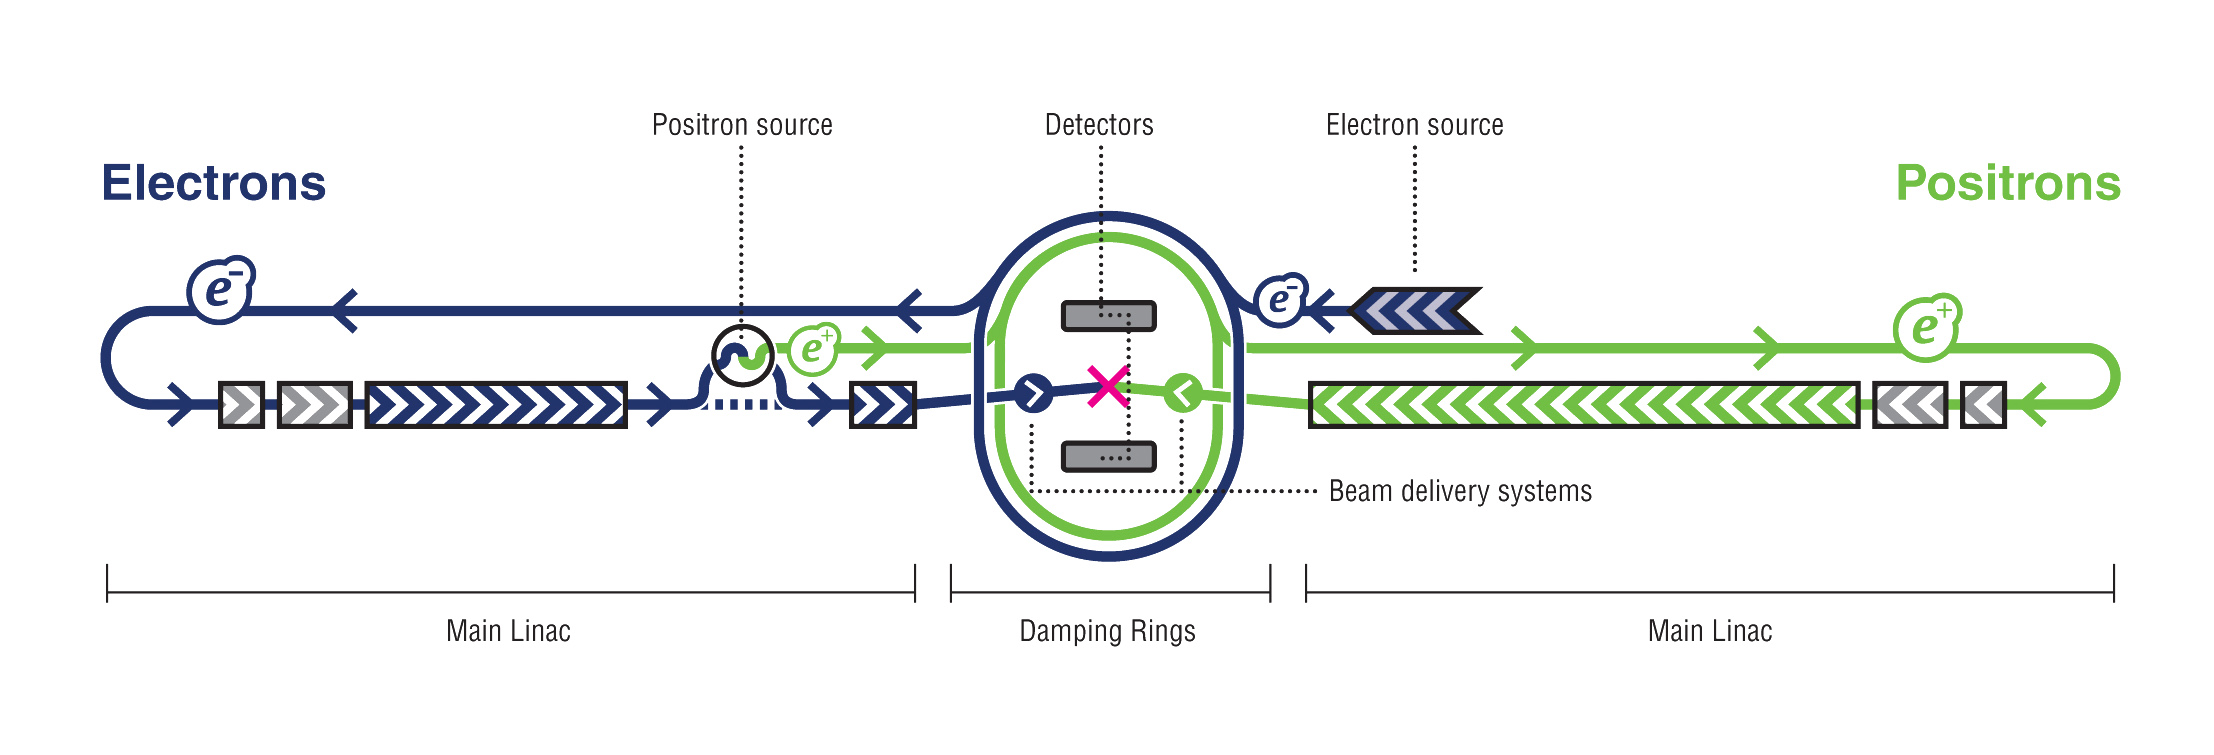
\includegraphics[width=0.95\textwidth]{graphics/ILC_scheme.jpg}
		\caption{\sl Vue sch\'ematique de l'ILC.}
		\label{fig:ILCSchemeF}
	}
\end{figure}

L’ILC devrait avoir deux d\'etecteurs, SiD et ILD, qui vont fonctionner de mani\`ere alternative.% pour assurer la v\'erification des r\'esultats.
Cette th\'es\`e est concentr\'e sur l'experiance ILD. 

L'International Large Detector (ILD) est un concept pour un détecteur multi-usages de haute précision. %, conçu pour atteindre les objectifs de physique de l'ILC~\cite{Behnke:2013lya}.
%La vue schématique de l'ILD est présentée dans la Figure~\ref {fig:ILCSchemeF}.
Comme montr\'e dans la vue schématique, Fig.~\ref {fig:ILDSchemeF}, ILD est compos\'e de plusieurs sous-d\'etecteurs, plac\'es les uns autour des autres:
\begin{itemize}
	\item un d\'etecteur de vertex \'a pixel multicouche (VTX);
	\item Le large de la tube de faisceau la trajectométrie est completée par un système de disque avec des pixels et des bandes de silicium;
	\item une ”Time Projection Chamber” (TPC) comme d\'etecteur des traces centrale;
	\item un calorim\`etre \'electromagn\'etique hautement granulaire (ECAL);
	\item un calorim\`etre hadronique hautement granulaire (HCAL);
	\item une bobine supraconductrice, qui cr\'ee un champ B axial de 3.5~Tesla.
	\item un d\'etecteur de muons et des queues des cascades hadroniques (TCMT).
\end{itemize}

\begin{figure}
	\centering
	\begin{subfigure}{0.5\textwidth}
		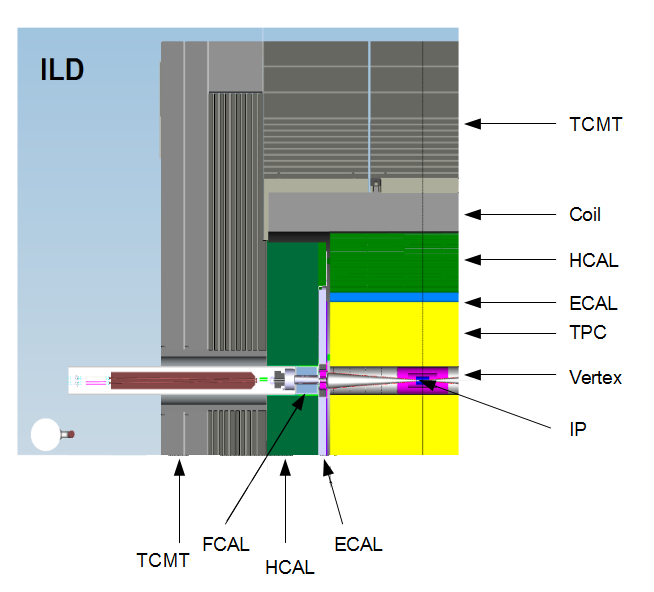
\includegraphics[width=0.95\textwidth]{graphics/ILD.png}
		
	\end{subfigure}% 
	\begin{subfigure}{0.5\textwidth}
		\centering
		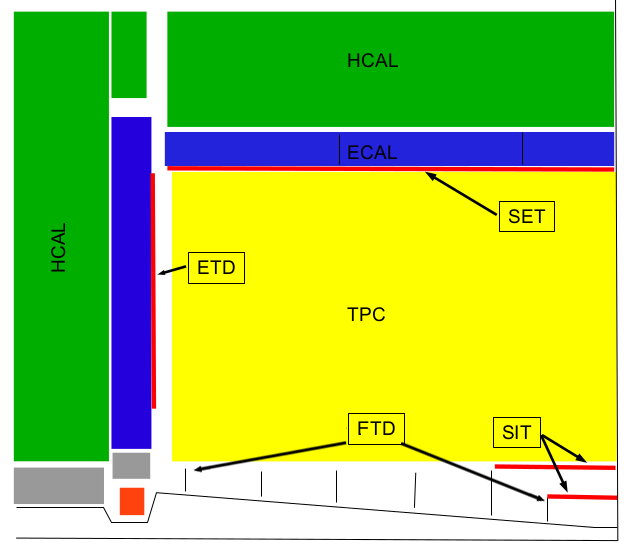
\includegraphics[width=0.9\textwidth]{graphics/ILDtracking.png}
		
	\end{subfigure}
	\caption{\sl Gauche: Vue sch\'ematique d'un quadrant de l'ILD. Droite: Gros plan sur les détecteurs internes.}
	\label{fig:ILDSchemeF}
\end{figure}
%-----------------------------------------------------------------------------
%-----------------------------------------------------------------------------
%-----------------------------------------------------------------------------
\newpage
\subsection*{Calorim\`etre \'electromagn\'etique silicium-tungst\`ene hautement granulaire}

Un calorim\`etre \'electromagn\'etique de silicium tungst\`ene (SiW-ECAL) est le
choix favorisé d'ILD.

La collaboration de CALICE (CAlorimetry for the LInear Collider Experiments) a construit et testé un prototype SiW-ECAL dont la vue schématique du prototype est présentée dans la Figure~\ref {fig:ECAL-schemeF}.

L'avantage du tungstène est sa grande longueur d'interaction ($\lambda_I = 96$\,mm), compar\'ee \`a son longueur de radiation  $X_0 = 3.5$\,mm. Cela conduit \`a une bonne s\'eparation longitudinale entre les photons et les hadrons. 
Des capteurs de silicium sous-divisés en pixels d'une taille de $1\times1$\,cm$^2$ servent comme mat\'eriau actif dans le prototype. 
\begin{figure}
	\centering
	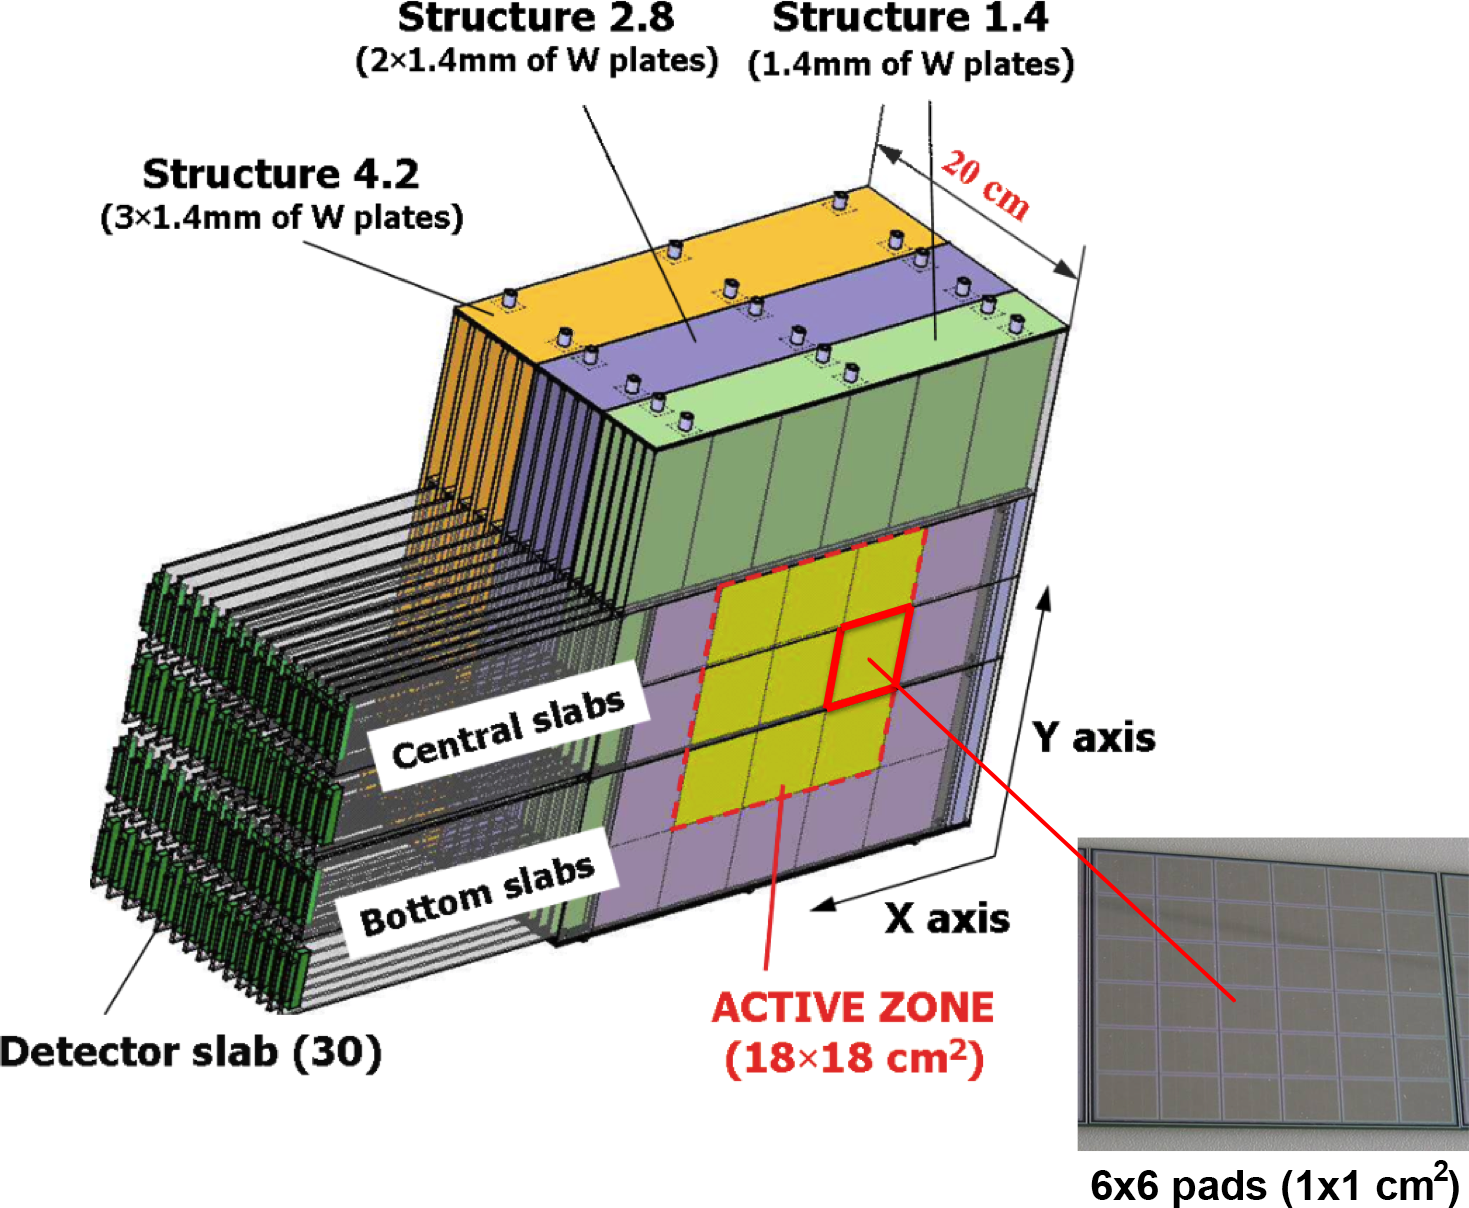
\includegraphics[width=0.55\textwidth]{ECAL/graphics/ecal-new.png}
	\caption{\label{fig:ECAL-schemeF} \sl  Vue sch\'ematique du \ecal.}
\end{figure}

Cette thèse présente une analyse de donnéés enregistrées avec le prototype du SiW-ECAL lors d'un campagne de test en faisceau au FNAL (Etats-Unis) en 2008.  
%-----------------------------------------------------------------------------
%-----------------------------------------------------------------------------
%-----------------------------------------------------------------------------
\newpage
\subsection*{L'algorithme de reconstruction de traces}
L'objectif principal de l'algorithme de traces developpé pour cette thèse est la détection de traces diffusées vers l'avant qui jaillissent de l'interaction entre les pions primaires et le matériau absorbant en absence d'un champ magnétique.

L'algorithme suit le sch\'ema d'ex\'ecution suivant:
\begin{itemize}
	\item La région d'interaction est identifiée par un critère topologique et séparée pour une analyse plus approfondie, voir Fig.~\ref{fig:testF};
	\item Les dépôts d'énergie restants sont regroupés dans des amas de pixels appellés  clusters dans la suite, voir Fig.~\ref{fig:democlusterF};
	\item Les clusters obtenus sont classés pour separer ceux qui ressemblent aux traces des signaux provenants du bruit résiduel; 
	\item Après la classification, les clusters qui appartiennent à la même particule secondaire   sont fusionnés dans une seule trace.
	
\end{itemize}
\begin{figure}
	\centering
	\begin{subfigure}{0.5\textwidth}
		\centering
		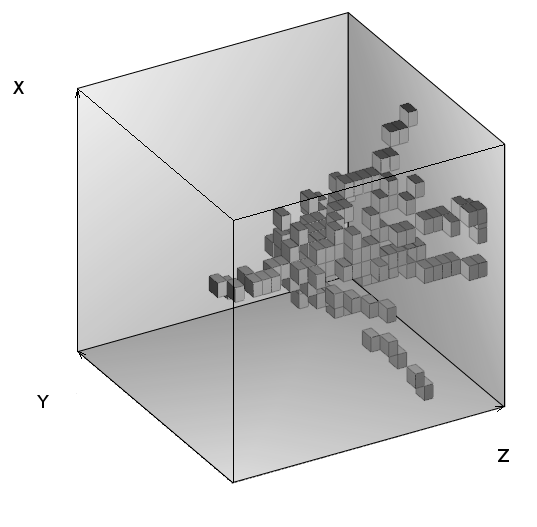
\includegraphics[width=.90\linewidth]{ECAL/graphics/before.png}
		\caption{\label{fig:beforeF} \sl avec région d'interaction.}
	\end{subfigure}% 
	\begin{subfigure}{0.5\textwidth}
		\centering
		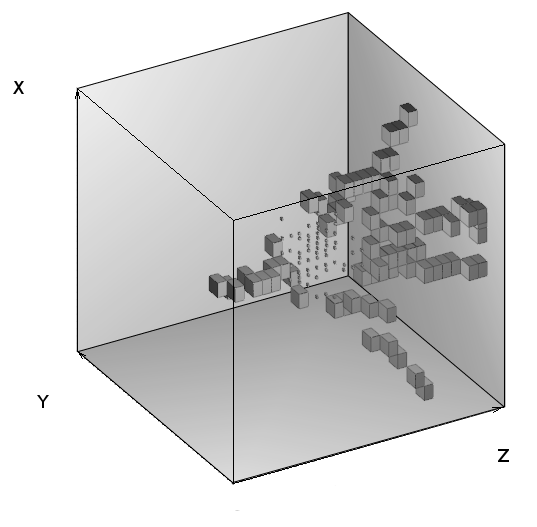
\includegraphics[width=.90\linewidth]{ECAL/graphics/after2.png}
		\caption{\label{fig:afterF} \sl sans région d'interaction.}
	\end{subfigure}
	\caption{ \sl Visualisation de l'interaction d'un pion primaire avec 10\,GeV d'\'energie enregistrée au FNAL 2008 avant \textit{(a)} et apr\'es suppression de la région d'interaction\textit{(b)}. }
	%Event 16-17 in Data10.root
	\label{fig:testF}
\end{figure}


\begin{figure}
	\centering
	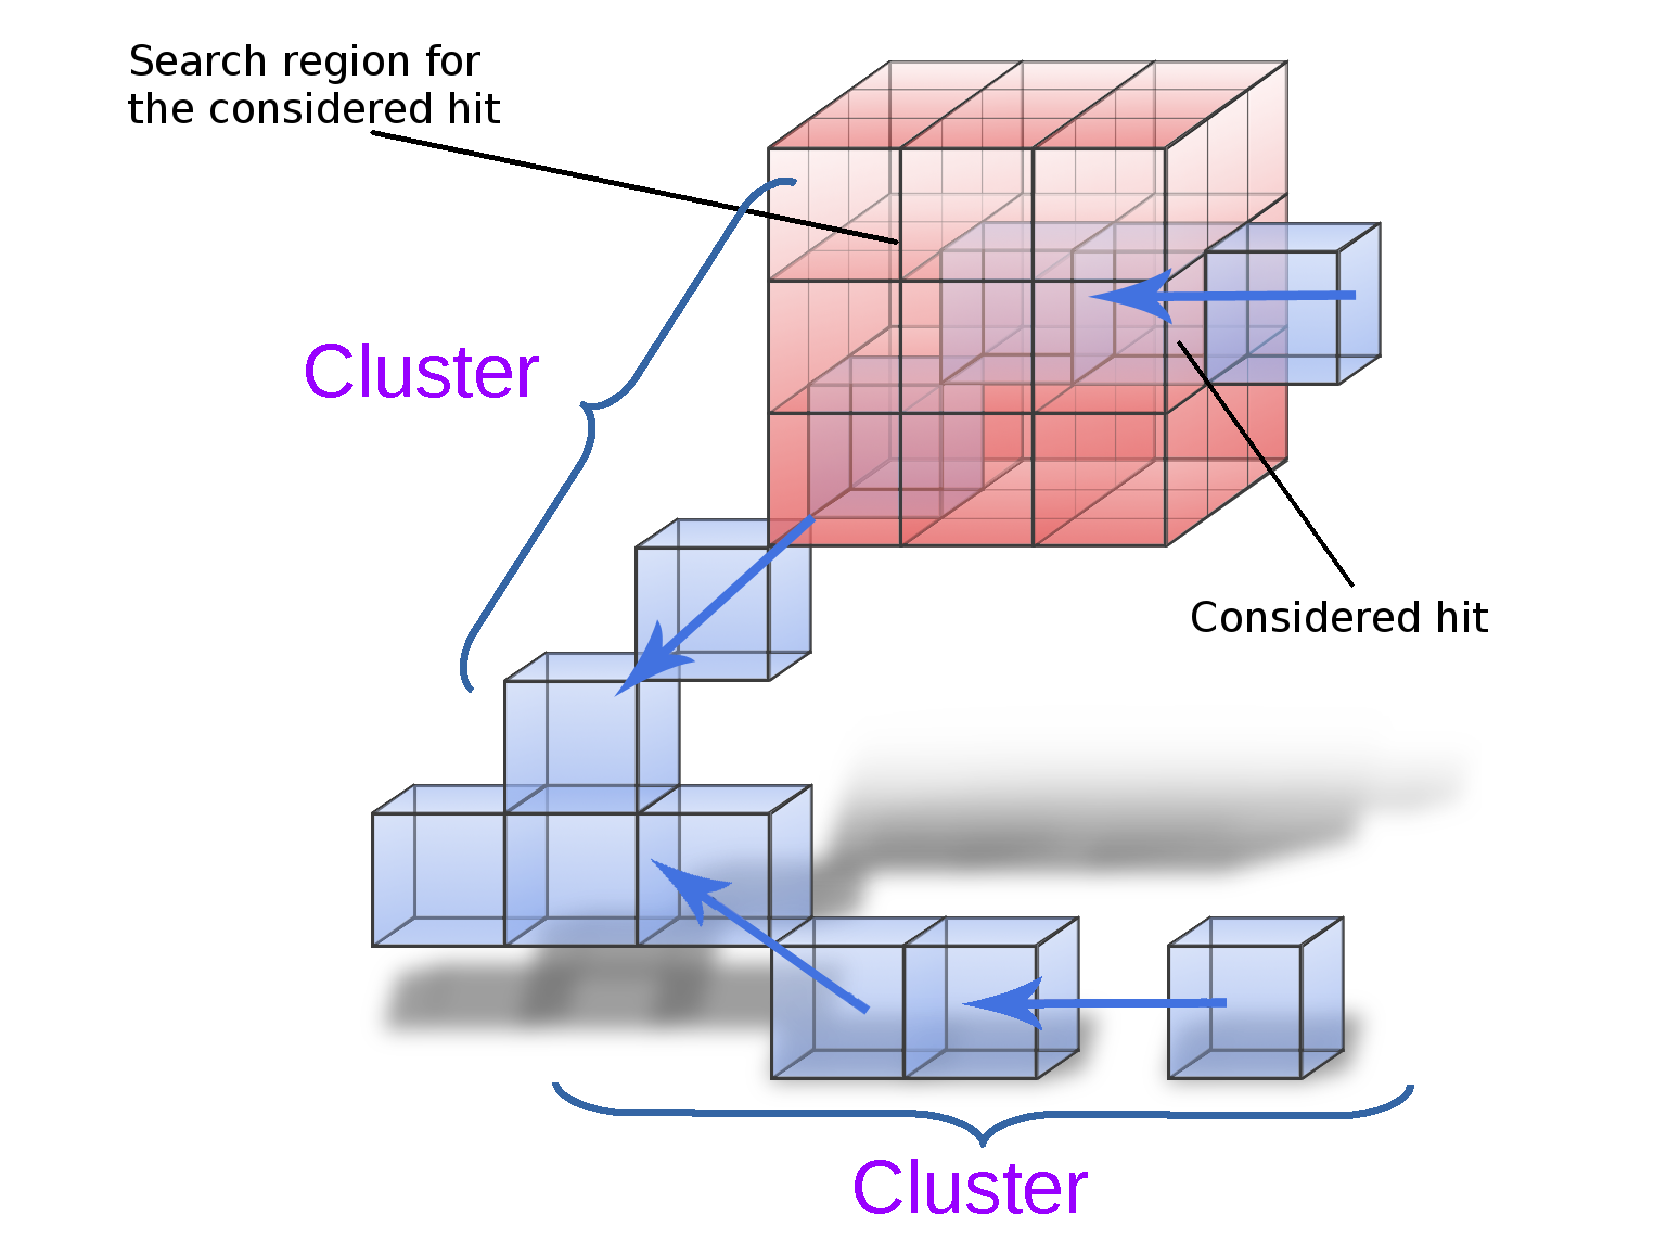
\includegraphics[width=0.55\textwidth]{ECAL/graphics/demo-v3.pdf}
	\caption{\label{fig:democlusterF} \sl Illustration des étapes de la clusterization. Les pixels actives sont représentés par des cubes bleus, et la zone de recherche pour les impacts adjacents est indiquée par des cubes rouges. Les flèches bleues indiquent la direction du flux de clusterization.}
\end{figure}

%-----------------------------------------------------------------------------
%-----------------------------------------------------------------------------
%-----------------------------------------------------------------------------
\newpage
\subsection*{Comparaison des simulations avec les données réelles}
La figure \ref{fig:irexampleF} montre les distributions du rapport entre l'énergie deposée dans la zone d'interaction sur l'énergie totale dans le detecteur. Les données sont comparées aux predictions de trois modèles de simulation des gerbes hadroniques proposés par le logiciel GEANT4.  
%La figure \ref{fig:irexampleF} montre les comparaisons des distributions d'énergie de la région d'interaction sur le dépôt d'énergie total $f_ {IR}$ entre les données et les trois listes de physique de {\sc Geant4}.
Le premier bac de chaque histogram  réprésent à la fraction d'événements pour laquelle aucune region d'interaction n'est trouvée par l'algorithme.


\begin{figure}
	\centering
	\begin{subfigure}{0.5\textwidth}
		\centering
		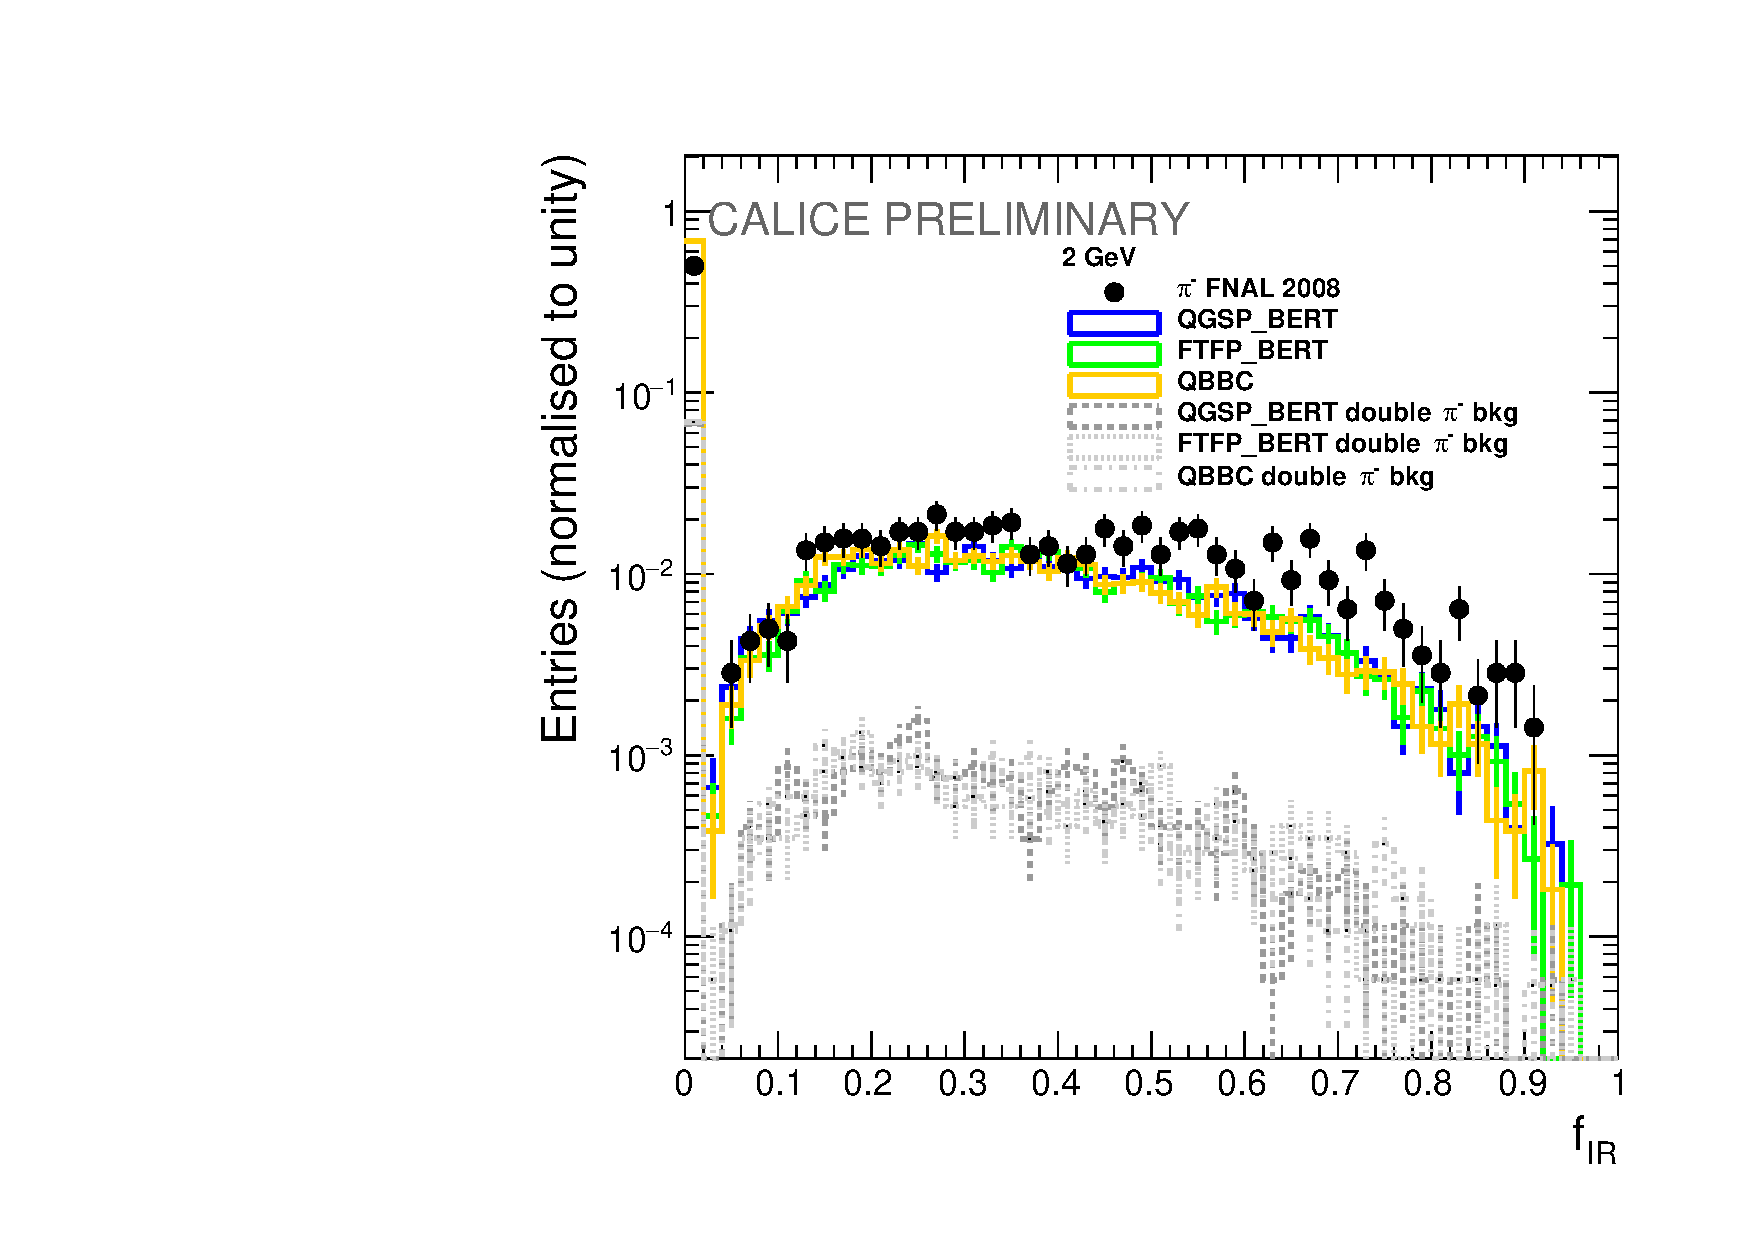
\includegraphics[width=.90\linewidth]{ECAL/plots/e-ir-2.pdf}
		\caption{\label{fig:efr2F} }
	\end{subfigure}% 
	\begin{subfigure}{0.5\textwidth}
		\centering
		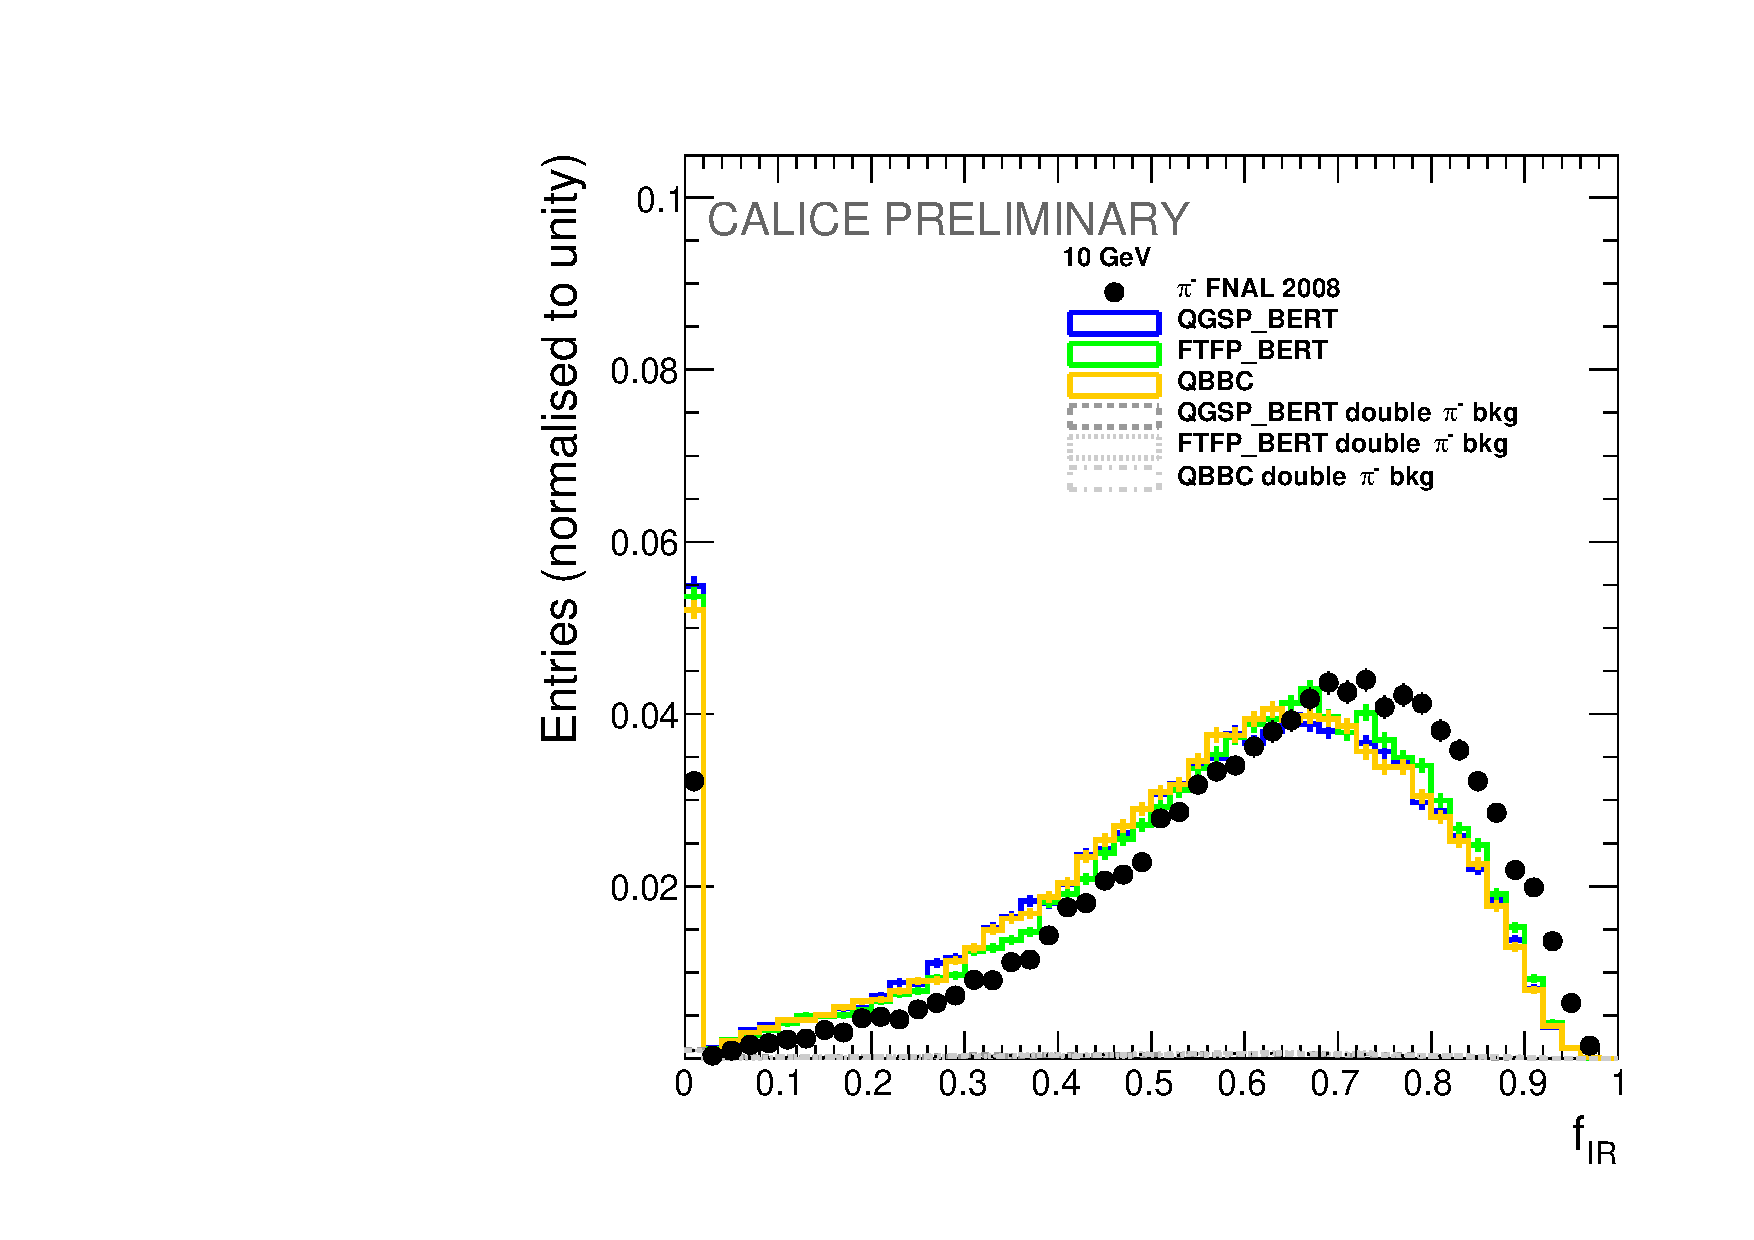
\includegraphics[width=.90\linewidth]{ECAL/plots/e-ir-10.pdf}
		\caption{\label{fig:efr10F} }
	\end{subfigure}
	\caption{\label{fig:irexampleF} \sl% {\bf Fig.~\ref{fig:efr2}: Remind me how the linear plot looks like} 
		Comparaison de $f_{IR}$ entre les données et les simulations pour trois {\sc Geant}4  listes physiques de l'\'energies 2 (a) et 10 (b) GeV de particule primordiale.}
\end{figure}

Dans la figure \ref{fig:irgraphF}, la valeur moyenne de $f_ {IR}$ est représentée en fonction de l'énergie du faisceau.% pour les énergies du faisceau de 2, 4, 6, 8 et 10 \, GeV.
La valeur moyenne de $f_{IR}$ prédit par les modèles de simulation est jusqu'à 20\% inférieure à celle observée dans les données.

\begin{figure}
	\centering
	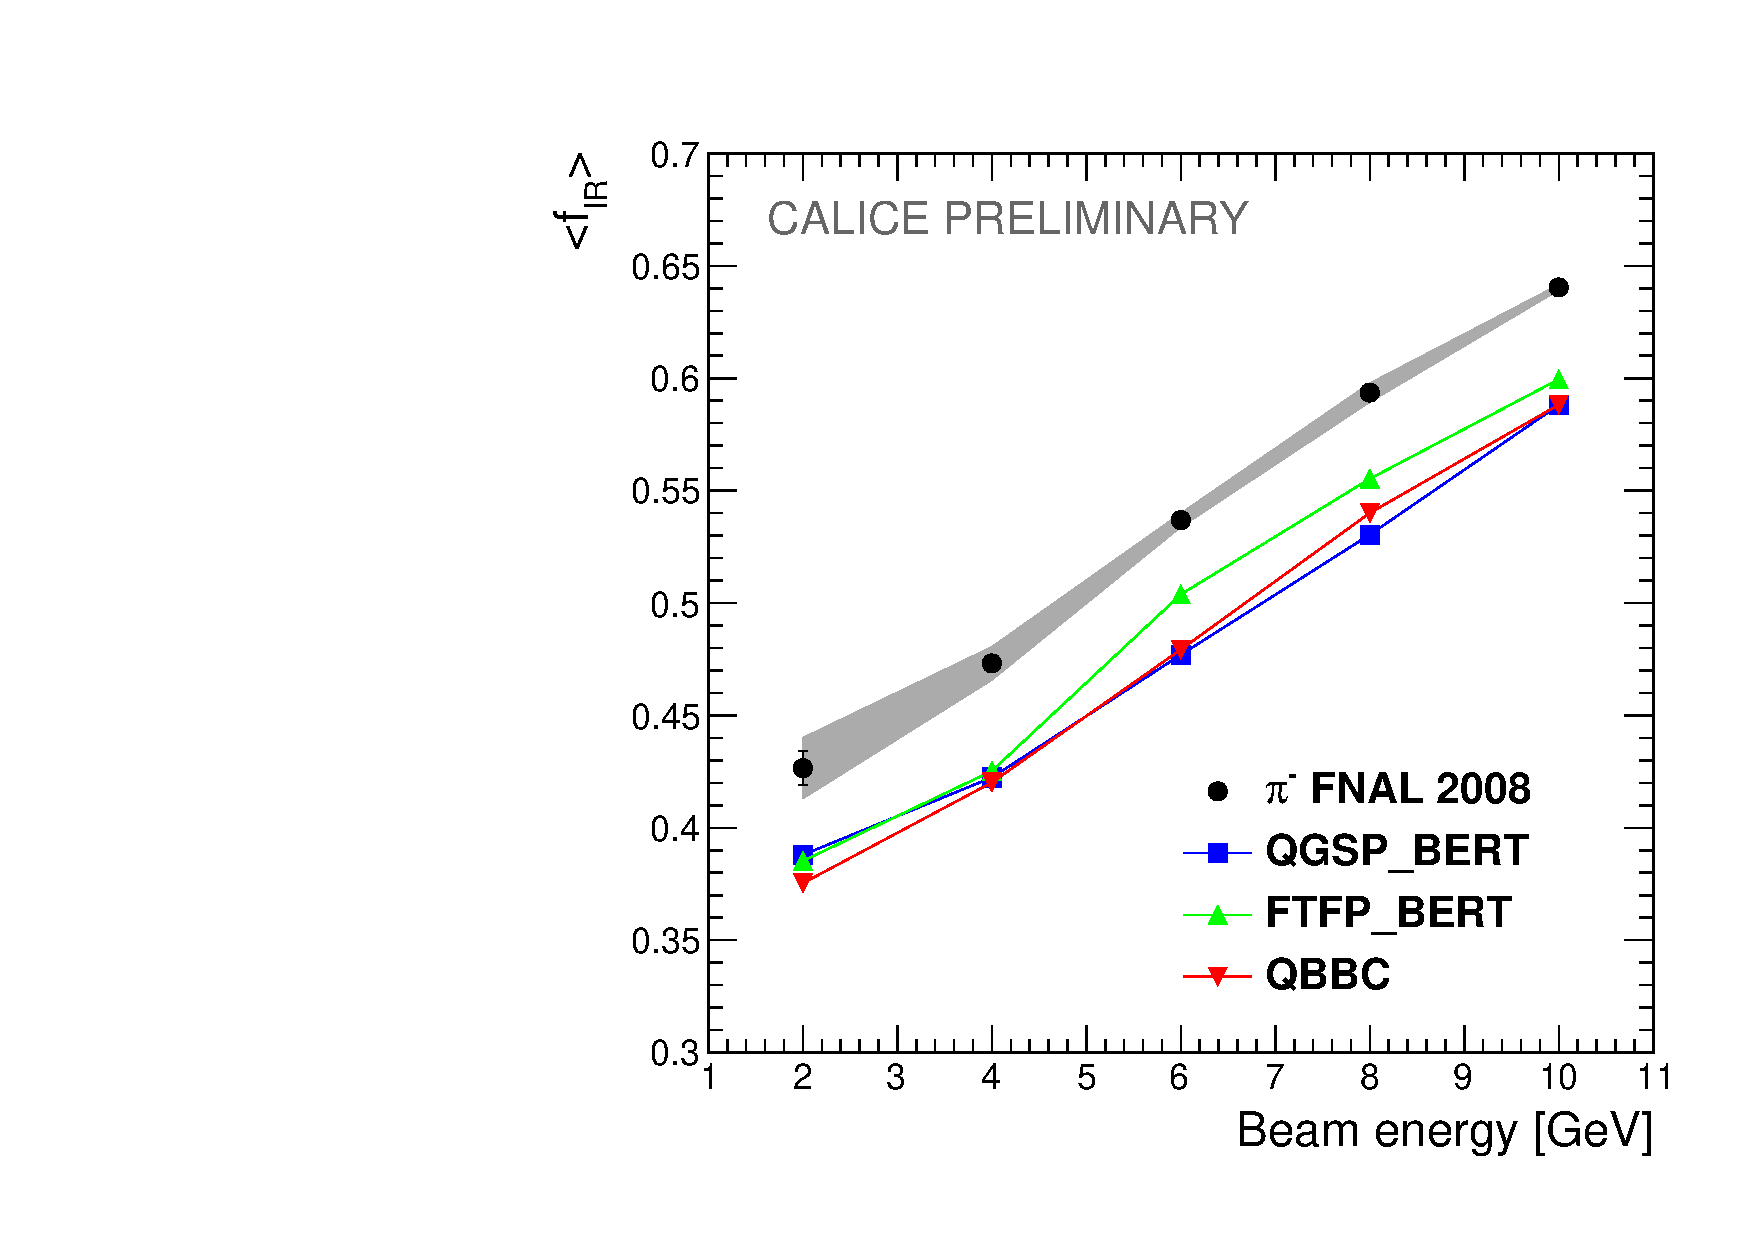
\includegraphics[width=0.5\textwidth]{ECAL/plots/e-ir-graph.pdf}
	\caption{\label{fig:irgraphF} \sl  Fraction moyenne du dépôt d'énergie dans la région d'interaction pour les données et les simulations  pour trois modèles de simulation proposés par le logiciel \geant\ en fonction de l'énergie du faisceau (2\,GeV à 10\,GeV).}
\end{figure}

%\begin{figure}
%	\centering
%	\begin{subfigure}{0.5\textwidth}
%		\centering
%		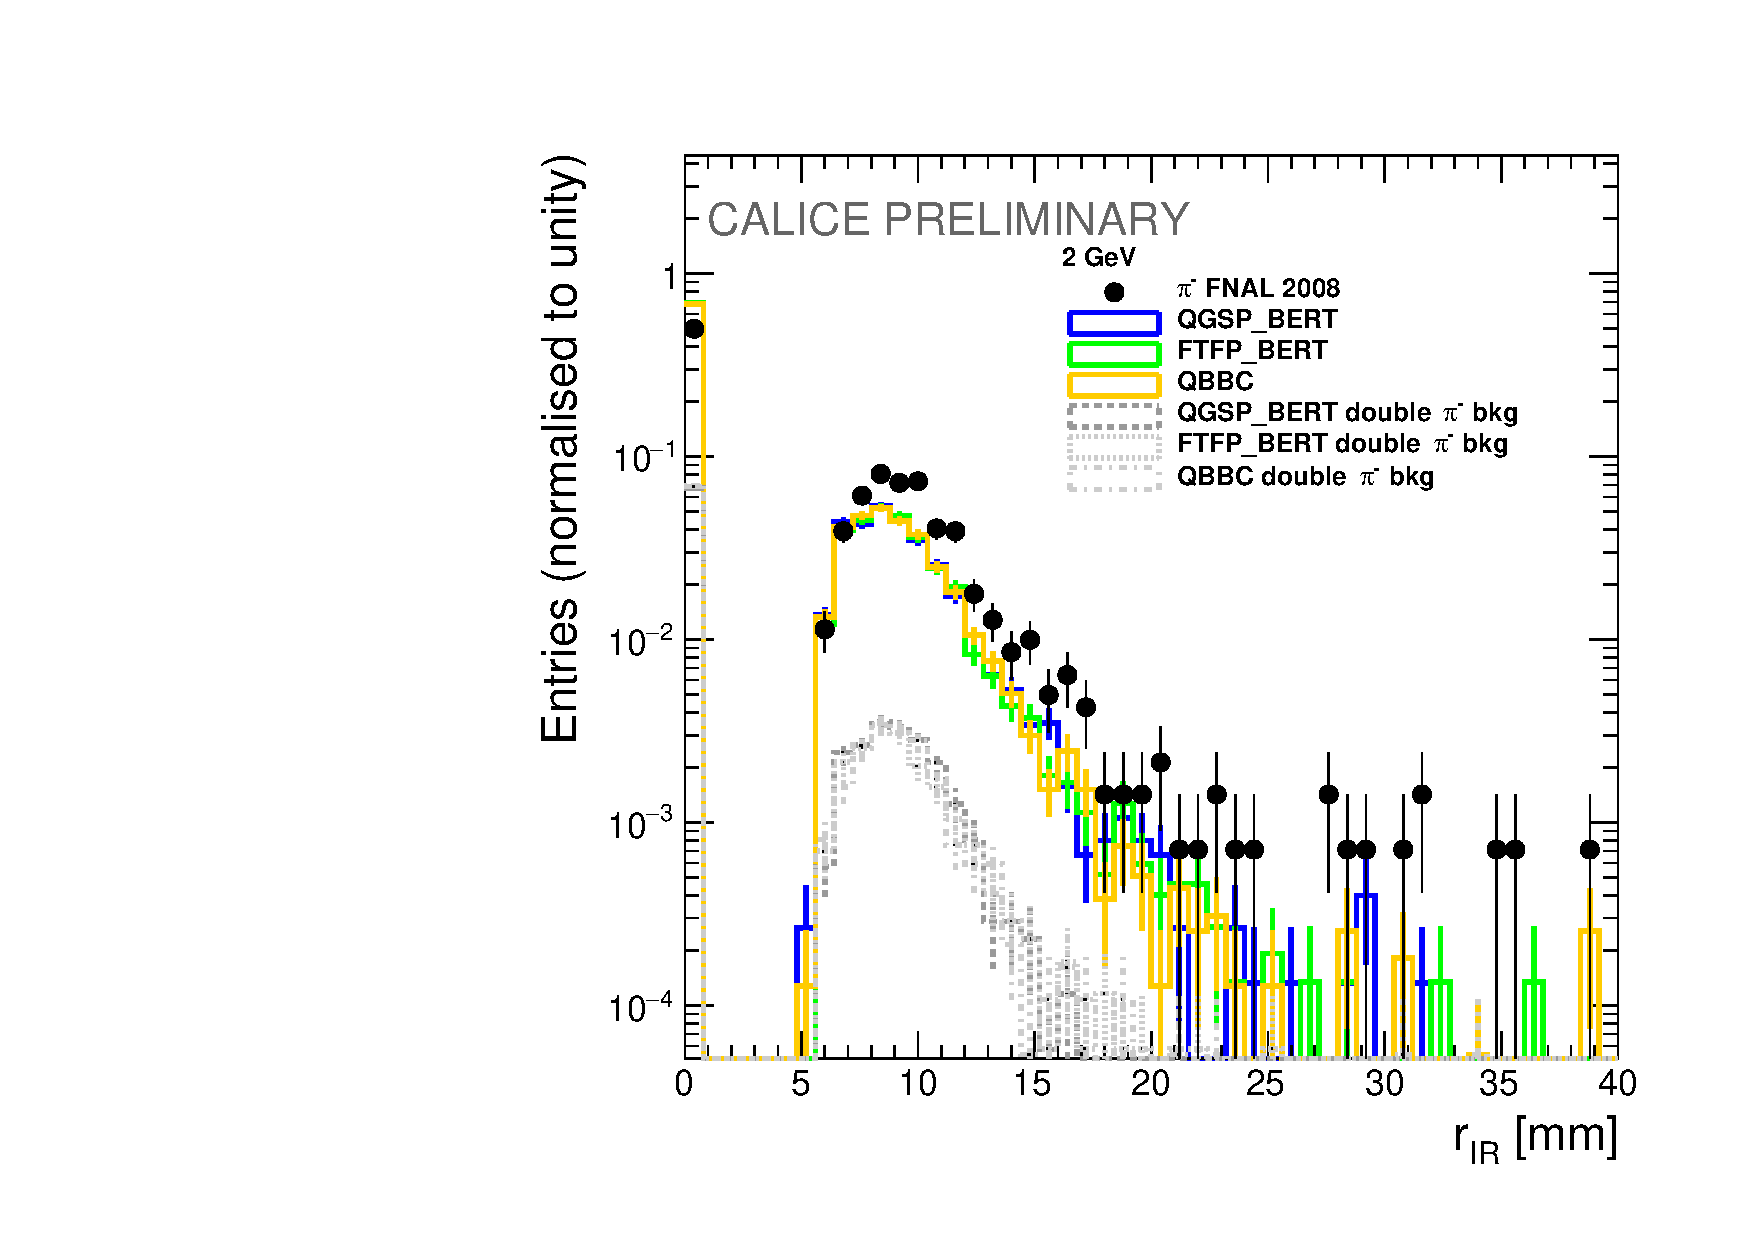
\includegraphics[width=.90\linewidth]{ECAL/plots/r-ir-2.pdf}
%		\caption{\label{fig:rir2F} }
%	\end{subfigure}% 
%	\begin{subfigure}{0.5\textwidth}
%		\centering
%		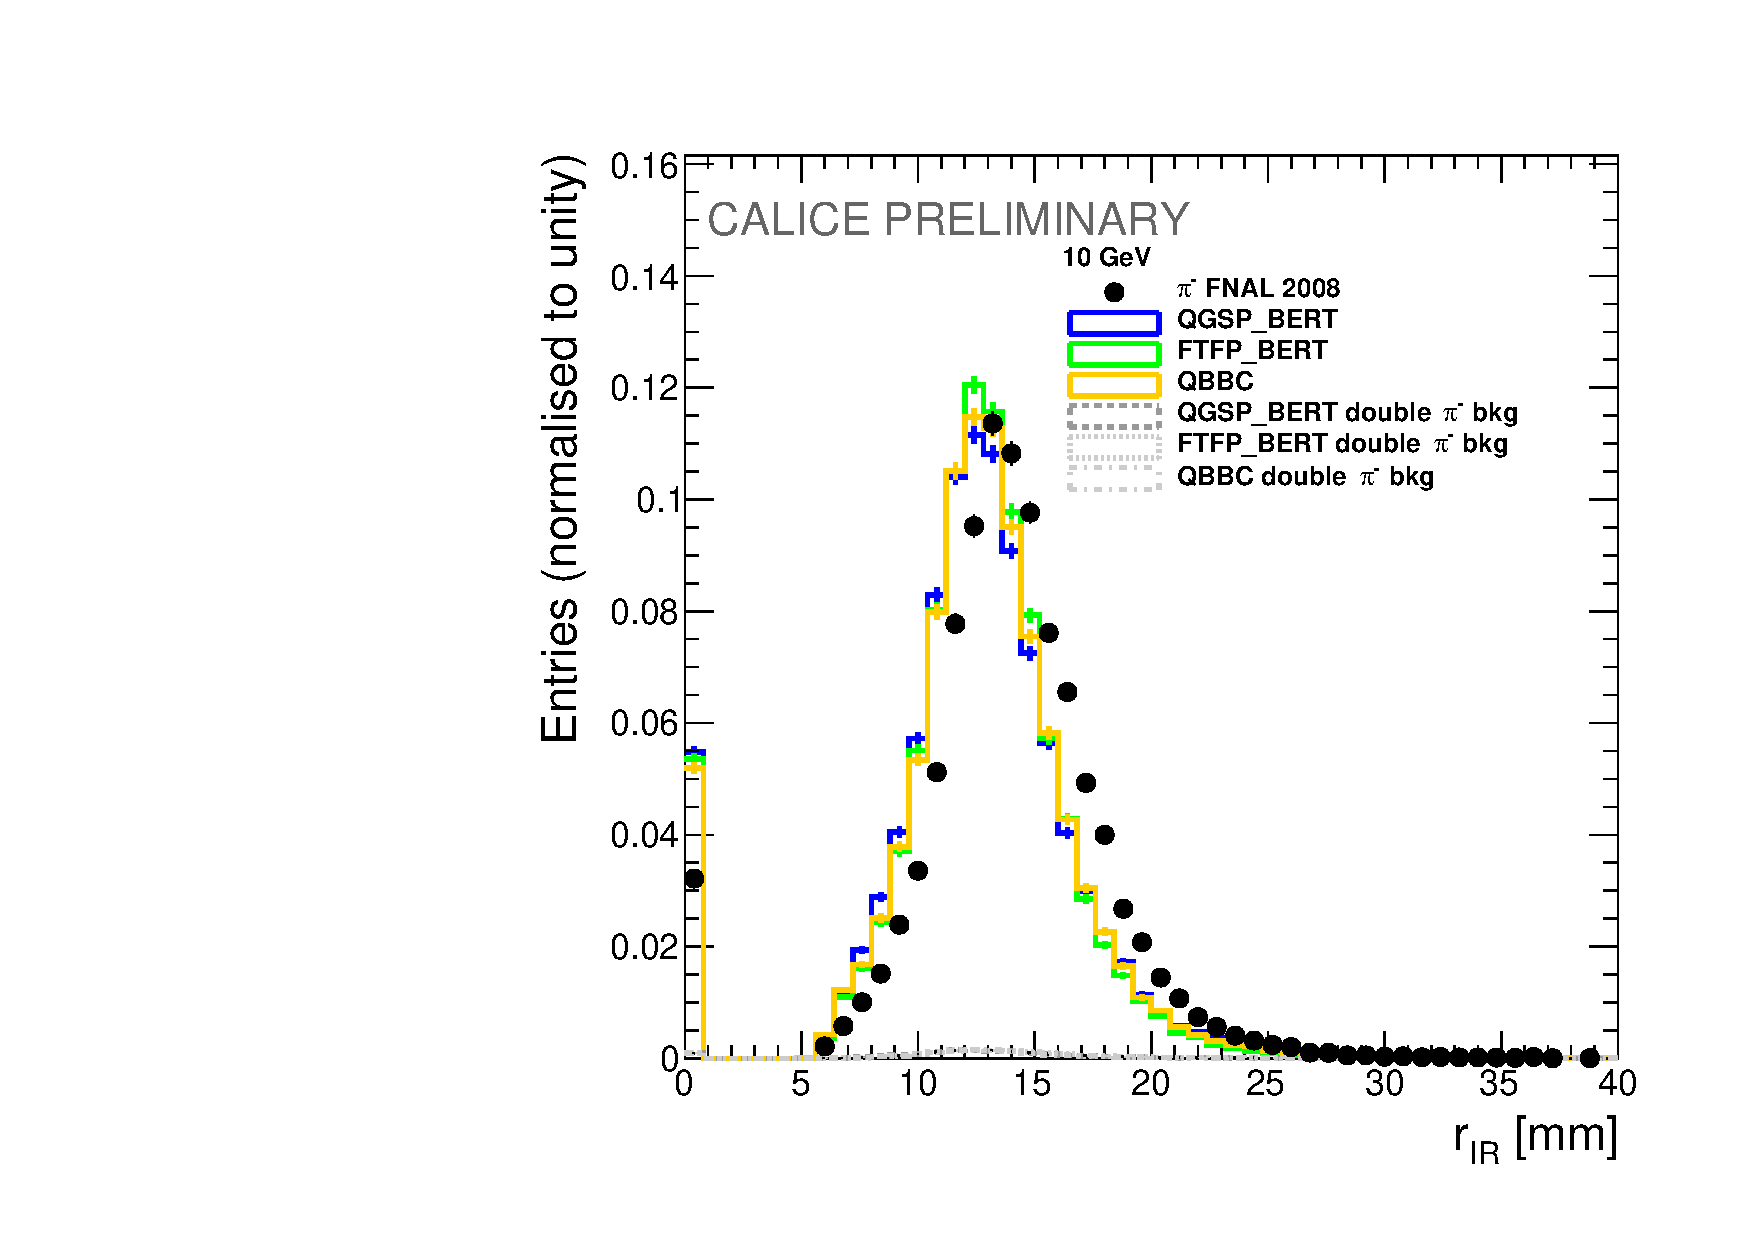
\includegraphics[width=.90\linewidth]{ECAL/plots/r-ir-10.pdf}
%	\end{subfigure}
%	\caption{\label{fig:rirexampleF} \sl %{\bf Same remark as for Fig.~\ref{fig:efr2} }
%		Comparaison de $r_{IR}$ entre les données et les simulations pour trois {\sc Geant}4  listes physiques de l'\'energies 2 (a) et 10 (b) GeV de particule primordiale.}
%\end{figure}

%\begin{figure}
%	\centering
%	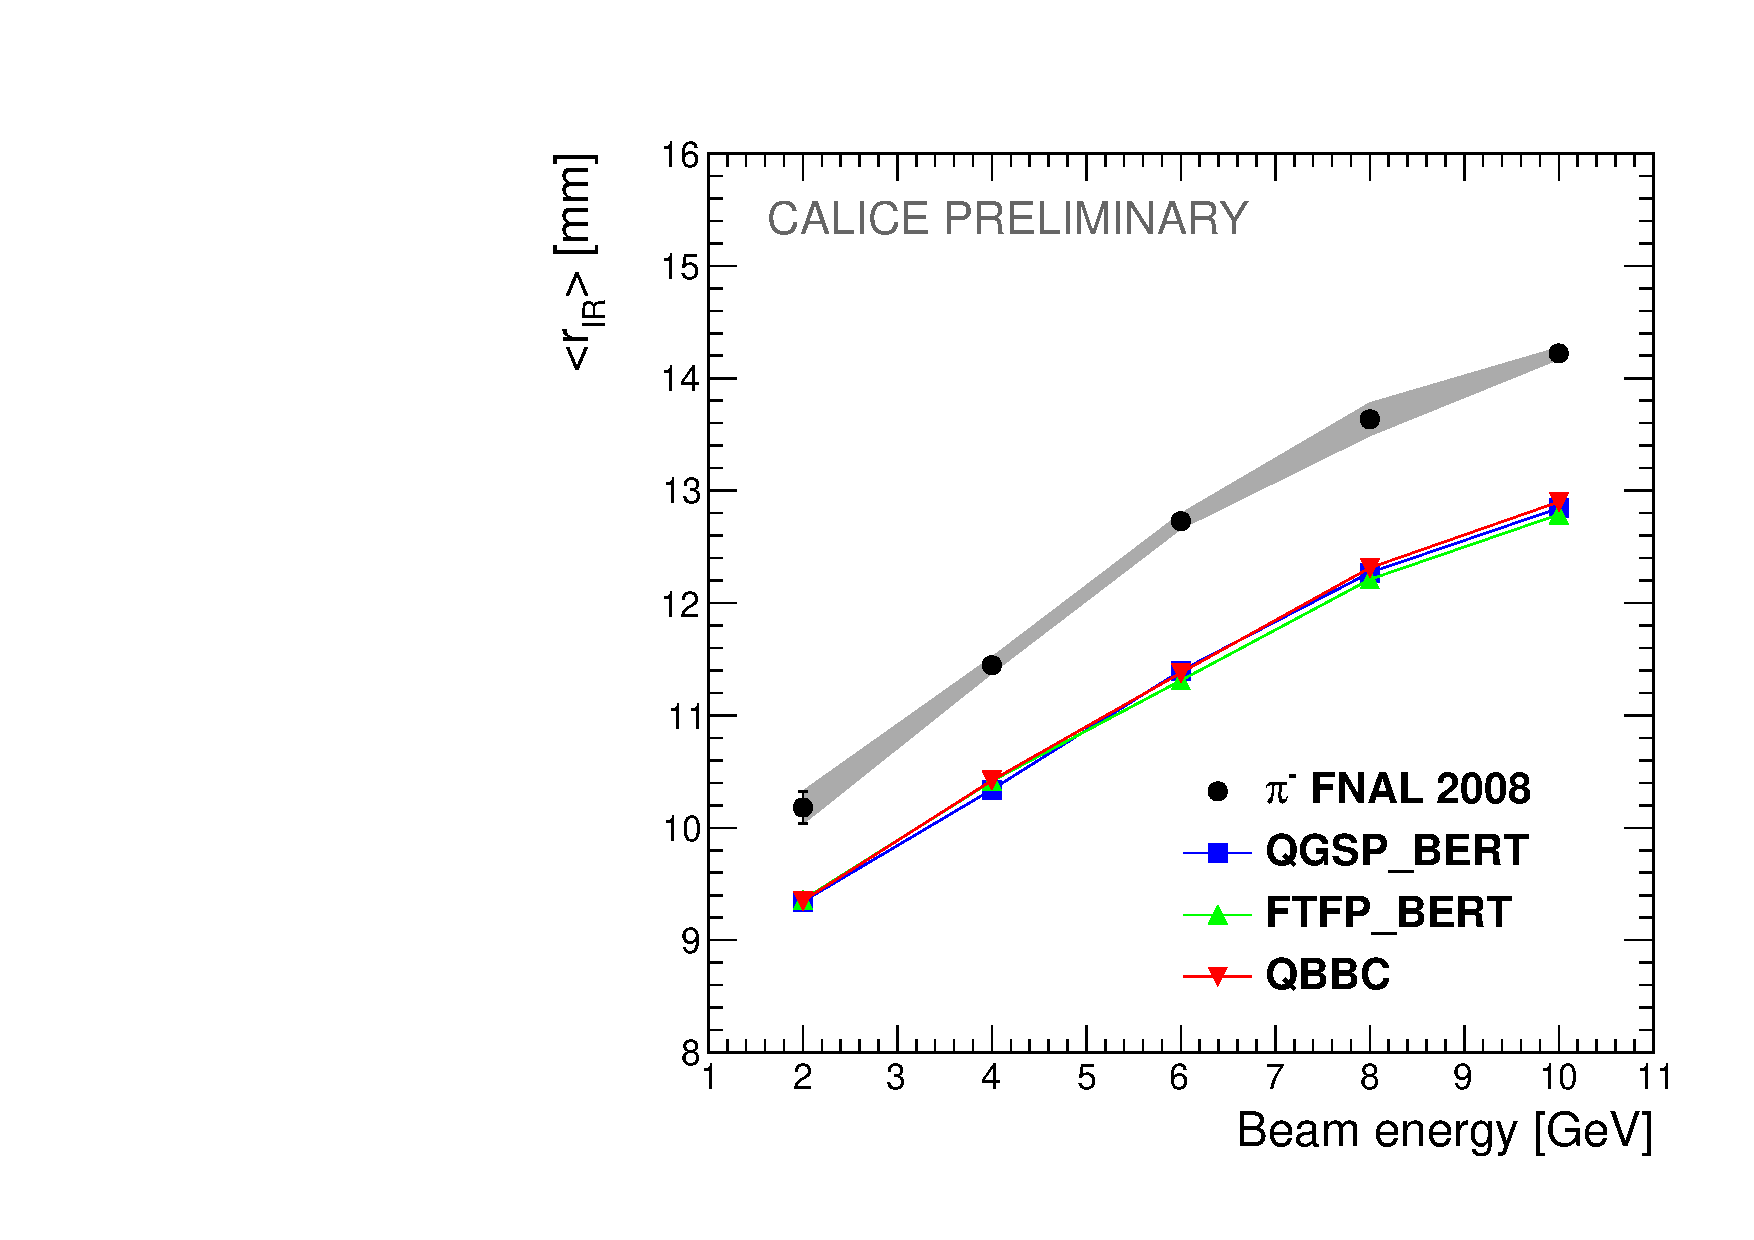
\includegraphics[width=0.5\textwidth]{ECAL/plots/r-ir-graph.pdf}
%	\caption{\label{fig:irrgraphF} \sl Radius lateral moyen de la région d'interaction pour les données et les simulations  pour trois listes physiques \geant\ comme une fonction de l'énergie du faisceau (2 \, GeV à 10 \, GeV).}
%\end{figure}

Un résultat central de l'analyse est le nombre de traces secondaires ($N_ {tracks}$). %et les observables en fonction de leurs propriétés.
Les distributions $N_ {tracks}$ sont présentées dans la Fig.~\ref{fig:NtrackF} pour  les données et les trois modèles de GEANT4 pour les énergies des pions primaires de 2 et 10 GeV. 

La valeur moyenne des nombres de traces est présentée en Fig. 1.9 en fonction de l'énergie des pions primaires. Les modèles de GEANT4 sont en bon accord avec les données à 2 et 10 GeV. Par contre ils sous-estiment le nombre de traces par environ 7\% entre ces deux valeurs.   

%Les trois listes de physique, présentées dans la Fig.~\ref{fig:fulltrackgraphF}, sous-estiment le nombre de traces secondaires de 7\% en moyenne inférieures à 10\,GeV et sont en accord avec les données à 10\,GeV.
\begin{figure}
	\centering
	\begin{subfigure}{0.5\textwidth}
		\centering
		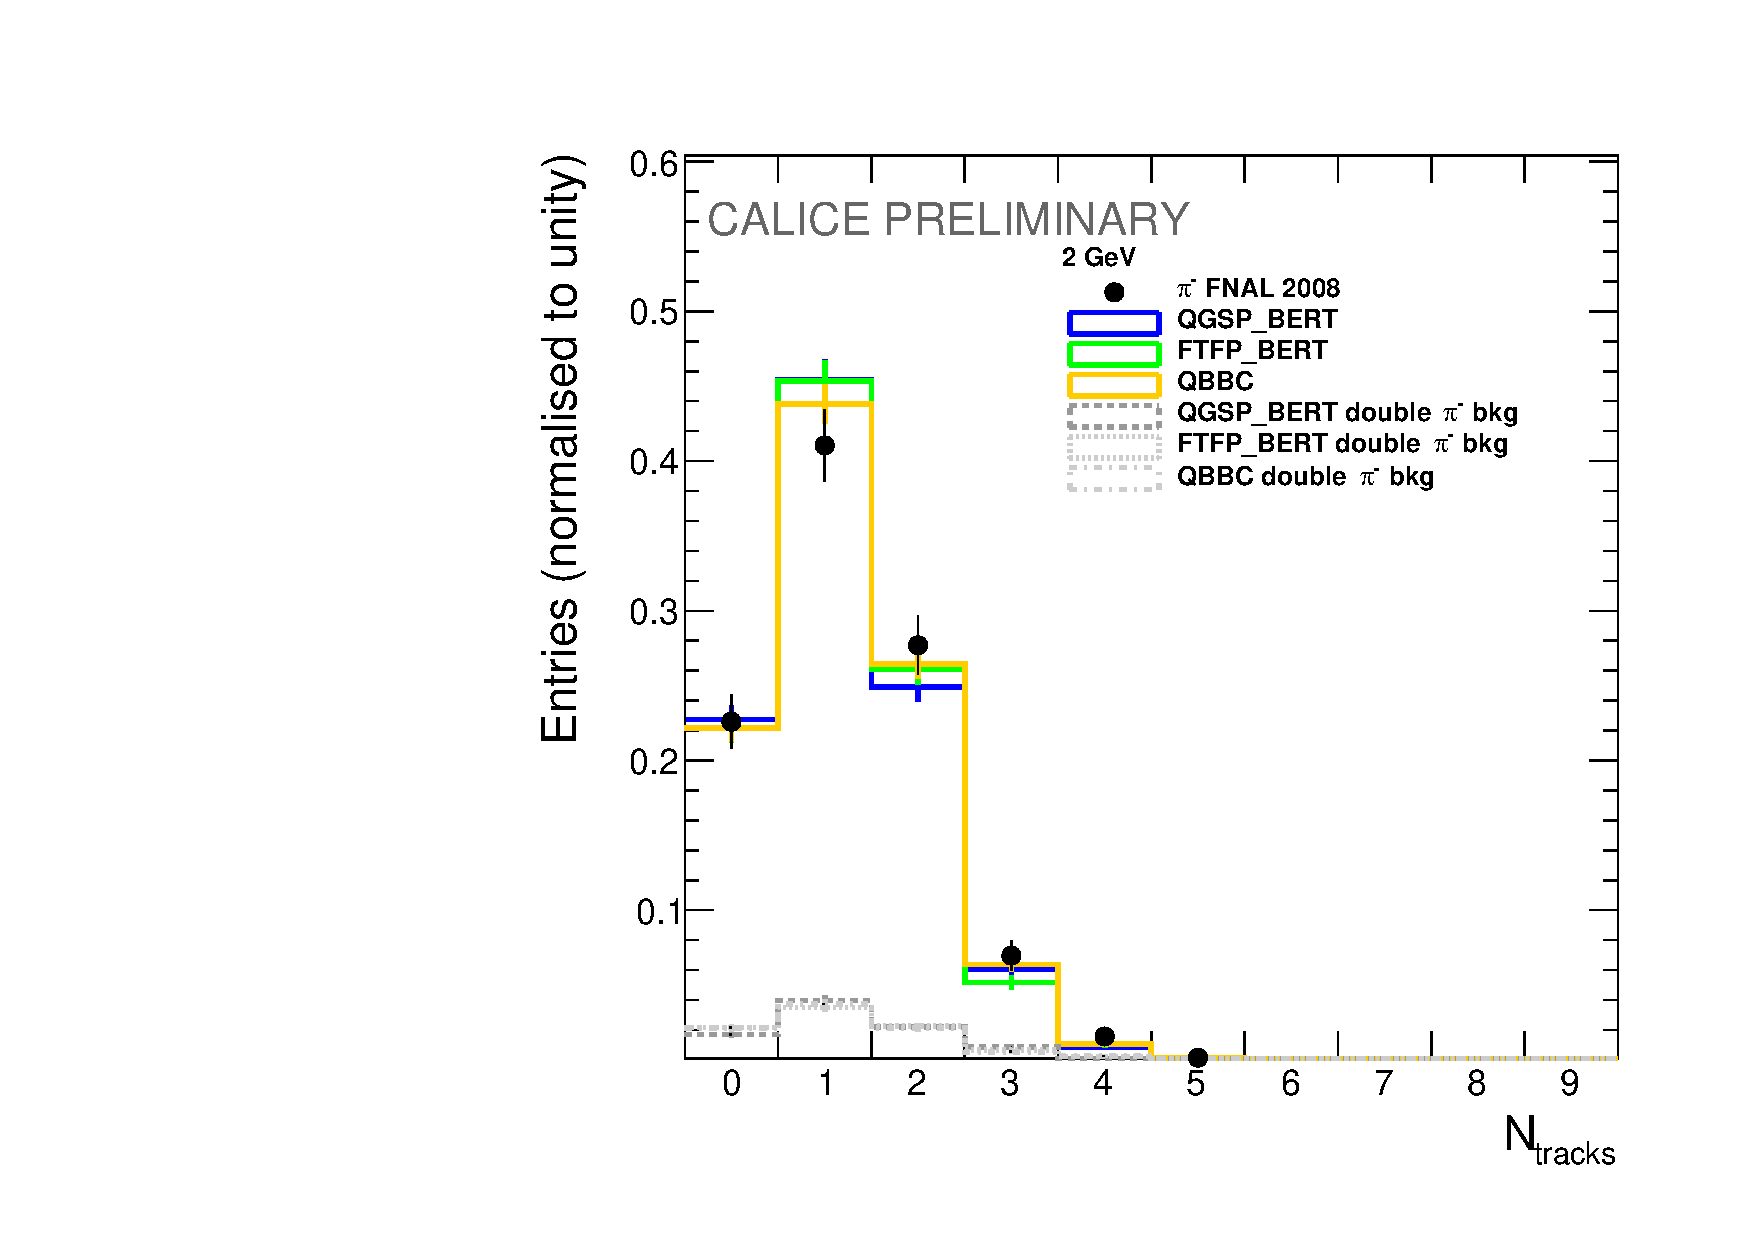
\includegraphics[width=.90\linewidth]{ECAL/plots/ntracks-2.pdf}
		\caption{\label{fig:tr2F} }
	\end{subfigure}% 
	\begin{subfigure}{0.5\textwidth}
		\centering
		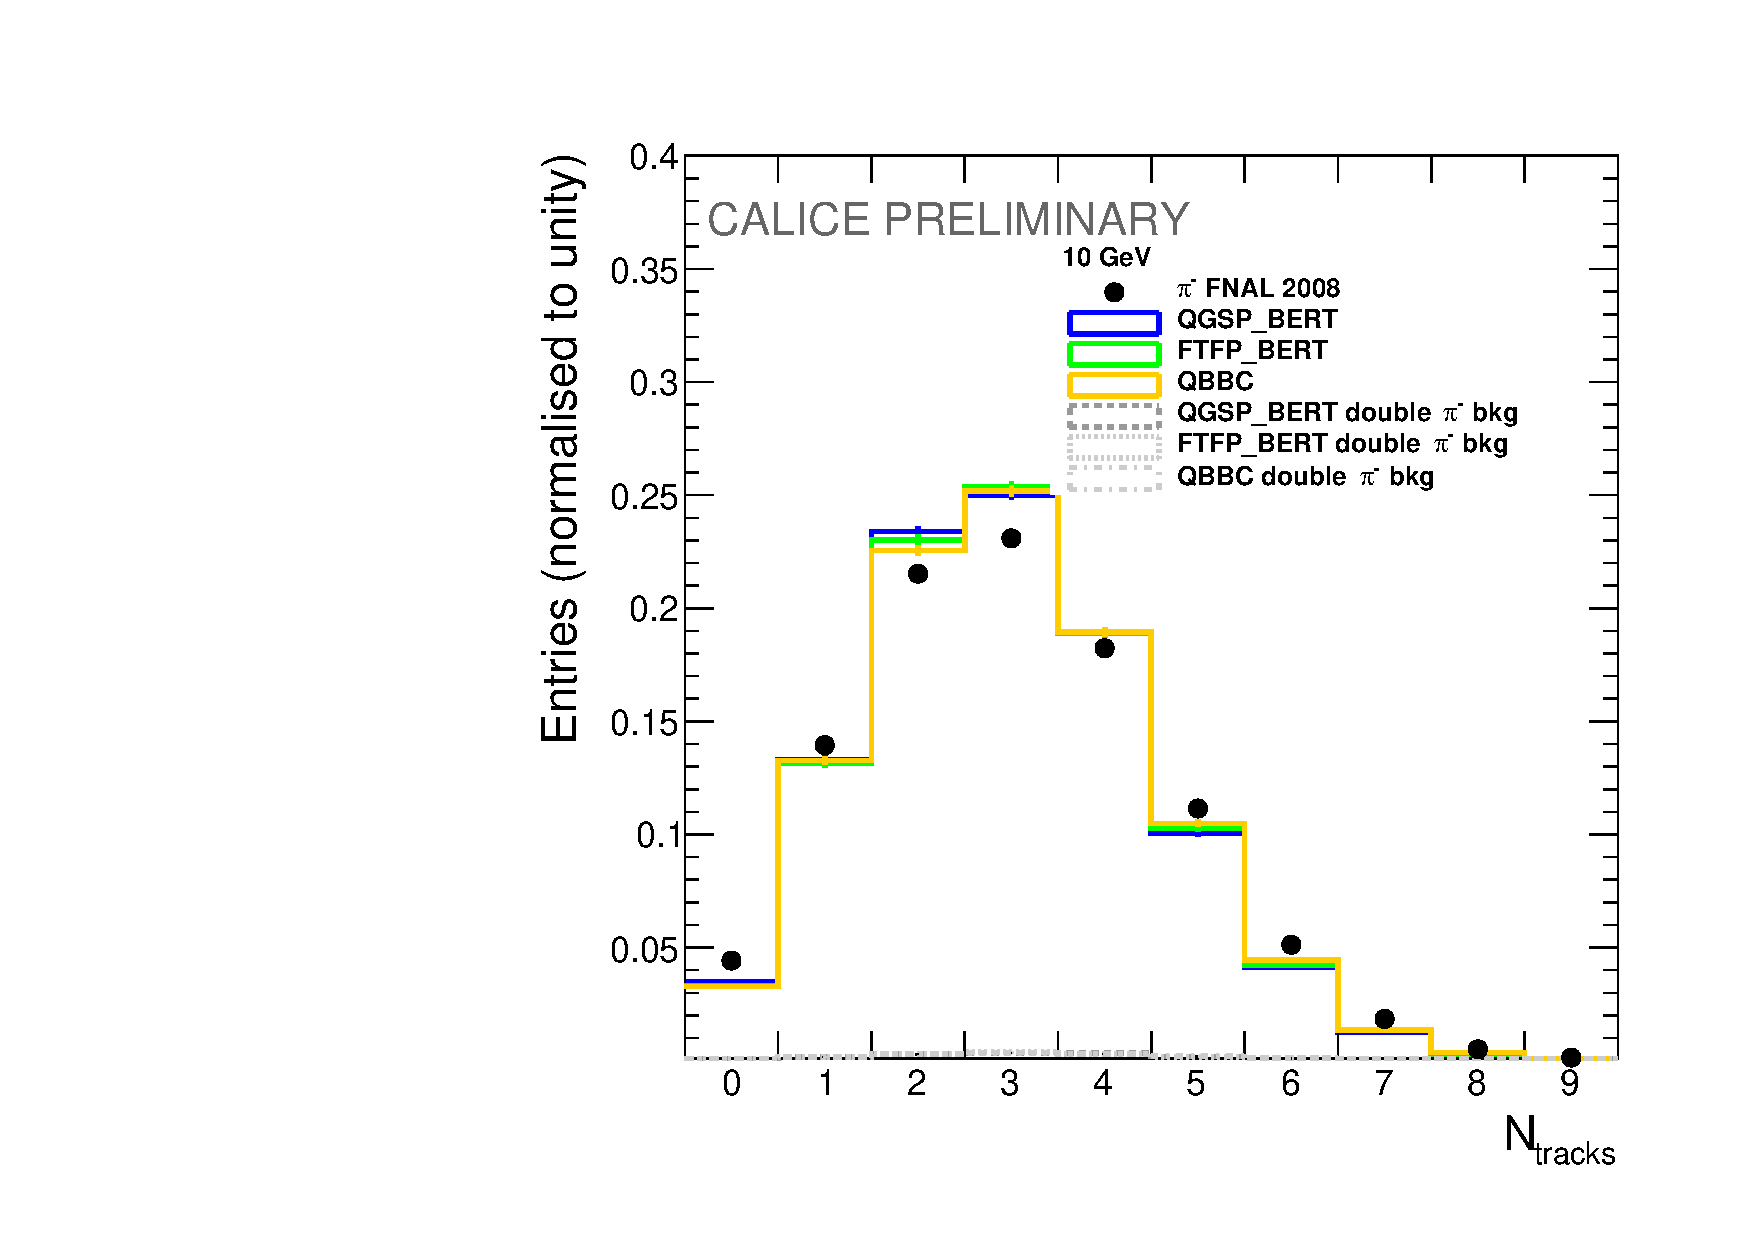
\includegraphics[width=.90\linewidth]{ECAL/plots/ntracks-10.pdf}
		\caption{\label{fig:tr10F} }
	\end{subfigure}
	\caption{\label{fig:NtrackF} \sl Comparaison de $N_{tracks}$ entre les données et les simulations pour trois modèles de simulation de  {\sc Geant}4. L'énergie du pion primaire est de 2 GeV (a) et 10 GeV (b).}
\end{figure}

\begin{figure}
	\centering
	\begin{subfigure}{0.5\textwidth}
		\centering
		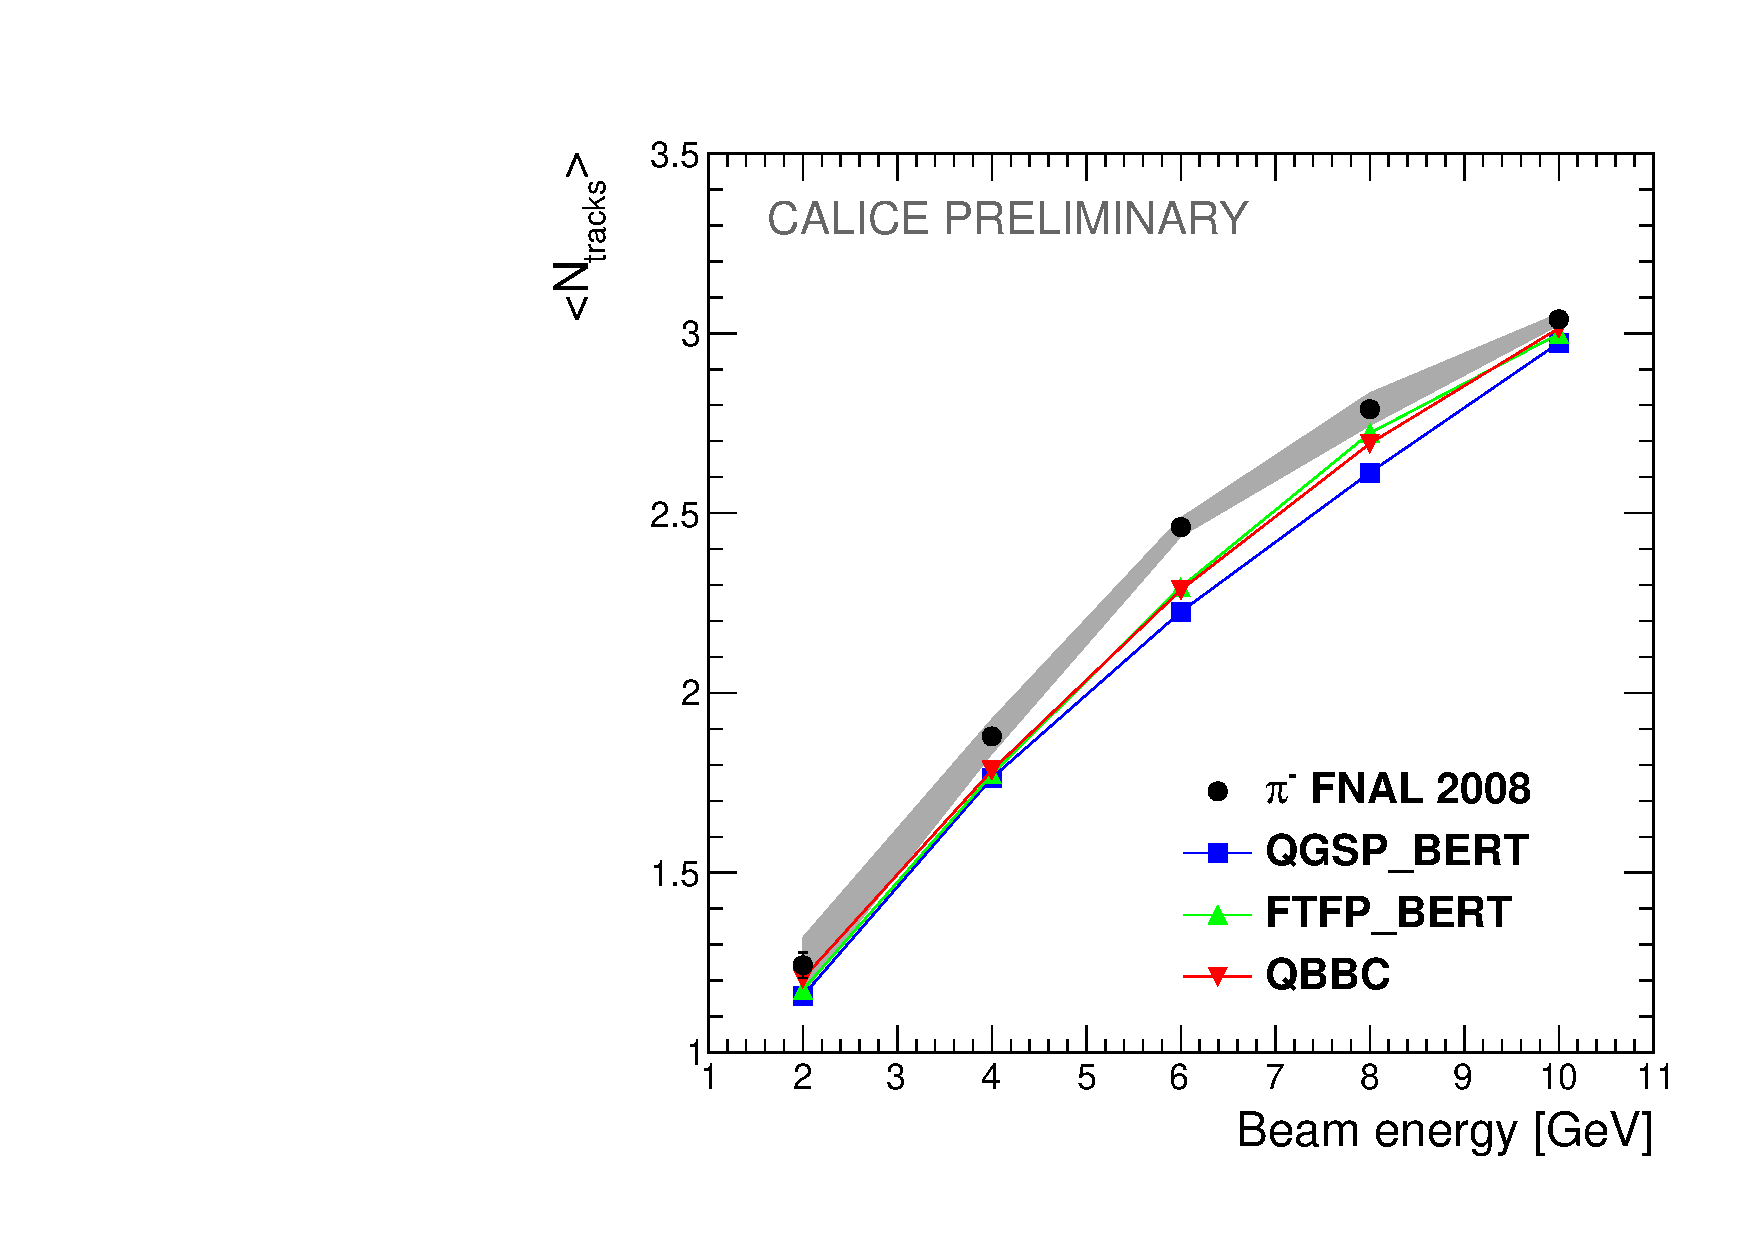
\includegraphics[width=.90\linewidth]{ECAL/plots/ntracks-graph.pdf}
		\caption{\label{fig:tracksgraphF} }
	\end{subfigure}% 
	\begin{subfigure}{0.5\textwidth}
		\centering
		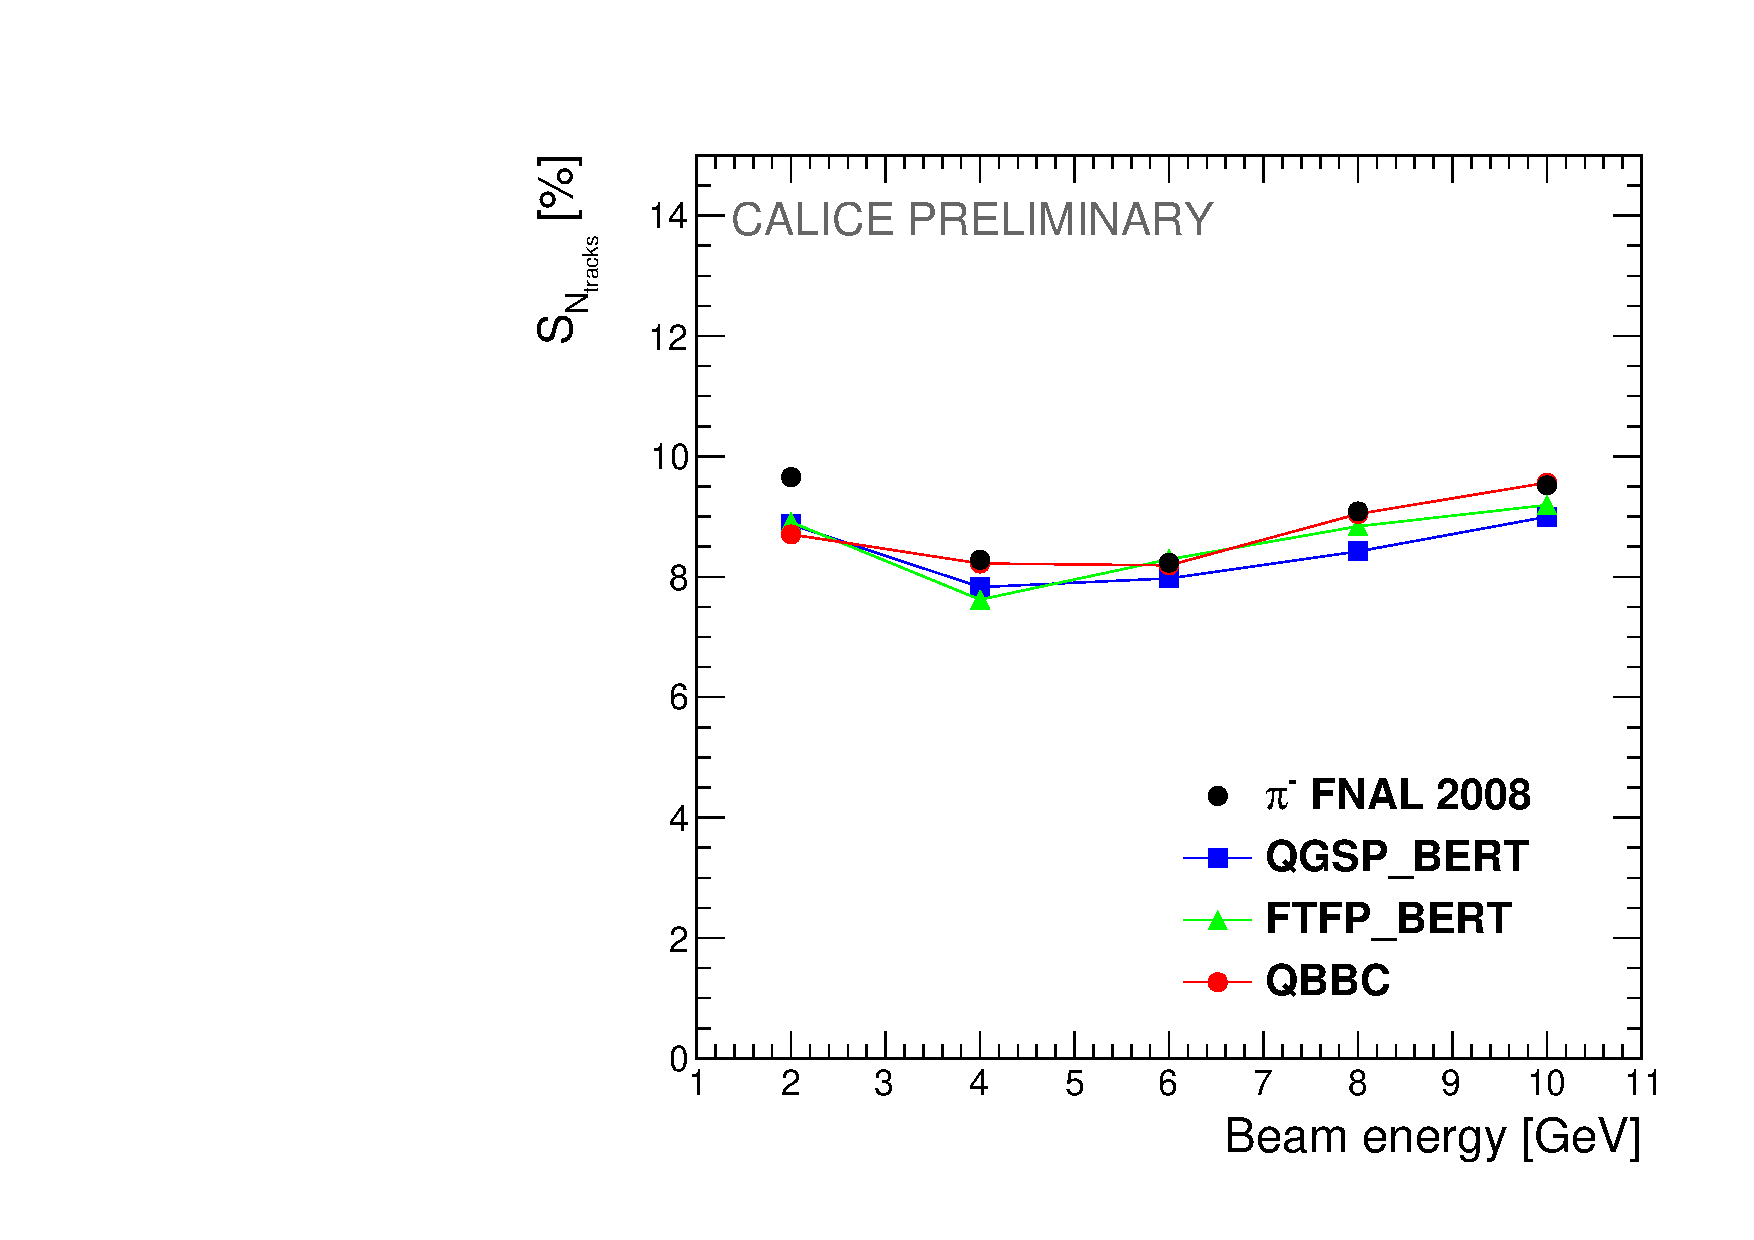
\includegraphics[width=.90\linewidth]{ECAL/plots/ntracks-graph-delta.pdf}
		\caption{\label{fig:dtracksgraphF}}
	\end{subfigure}
	\caption{\label{fig:fulltrackgraphF} \sl Nombre moyen des traces trouvées pour les données et les simulations  pour trois listes physiques \geant\ en fonction de l'énergie du faisceau (2\,GeV à 10\,GeV). }
\end{figure}


%-----------------------------------------------------------------------------
%-----------------------------------------------------------------------------
%-----------------------------------------------------------------------------
\newpage
\subsection*{Les quarks top et bottom \'a l'ILC}

La masse du quark top est comparable à la valeur d'anticipation du vide électrofaible et elle est beaucoup plus grande que les masses de toutes les autres particules connues aujourd'hui et notammeent de celles des bosons de la force électrofaible.
\c Ca fait du top quark un sujet de nombreuses théories de la nouvelle physique.

Des mesures précises des couplages de quarks lourds sont donc des pistes prometteuses de la recherche indirecte pour des nouvelles particules et la discrimination entre différentes théories.

Cette section porte sur la production électrofaible des paires de quarks top et bottom.

Les paires de fermions $f$ sont produites au vertex $f\bar{f}X$, où $X$ représente des bosons vectoriels neutres, le photon ou le boson de $Z^0$. Le courant au $f\bar{f}X$ vertex peut être exprimé comme suit:
\begin{equation}
\Gamma^{f\bar{f}X}_\mu (k^2,q,\bar{q}) = ie\{ \gamma_\mu (F^X_{1V}(k^2) + \gamma^5 F^X_{1A}(k^2)) - \frac{\sigma_{\mu\nu}(q-\bar{q})^\nu}{2m_f}(iF^X_{2V}(k^2) + \gamma^5 F^X_{2A}(k^2)) \},
\end{equation}
où $k^2= (q+\bar{q})^2$ est la quadri-impulsion au carré du boson du vecteur échangé, $q$ et $\bar{q} $ sont les quadri-impulsions du fermion $f$ et du antifermion $\bar{f}$ et $m_f$ est la masse des deux. Les $\gamma_\mu$ et $\gamma_5$ sont les matrices de Dirac, et $\sigma_{\mu\nu} = i/2(\gamma_\mu\gamma_\nu - \gamma_\nu\gamma_\mu)$.

Finalement, les $F$ sont des facteurs de forme, qui contiennent les corrections quantiques du vertex. Au niveau Born les $F$ prennent les valeurs suivantes:  
%Les valeurs de \sm\ du facteurs de forme sont les suivantes:
\begin{equation}
F^{f\gamma}_{1V} = Q^{f}, \ F^{f\gamma}_{1A} = 0, \ F^{fZ}_{1V} = \frac{I^f - 2Q^f\sin^2\theta_W}{2\cos\theta_W\sin\theta_W}, \ F^{fZ}_{1A} = - \frac{I^f}{2\cos\theta_W\sin\theta_W},
\label{formula:SMformFactors_3F}
\end{equation}
et toutes les facteurs $F_2$ sont 0. Dans l'équation~\ref{formula:SMformFactors_3F} $I^f$ est  l'isospin faible, $I^t = 1/2$ pour top et $I^b = -1/2$ pour quark bottom  et $Q^f$ est la charge electrique, $Q^t = 2/3$ et $Q^b = -1/3$.


Le facteurs de forme sont liés aux couplages des fermions des hélicités droite et gauche au boson de $Z^0$. Il est $g_L = F^Z_{1V} - F^Z_{1A}$  et $gR = F^Z_{1V} + F^Z_{1A}$.
Les resultats obtenus dans cette these sont exprimés en termes de $g_L$ et $g_R$.  
%The form factors are related to fermion couplings with left and right-handed helicity to $Z^0$ boson:
%La définition suivante des couplages gauches et droites $Z^0b\bar{b}$ est utilisée tout au long de la thèse: 
\begin{equation}
%g_L^Z = (F_{1V}^Z - F_{1A}^Z), \  g_R^Z = F_{1V}^Z + F_{1A}^Z, 
g_L^Z = I^f - Q^f\sin^2\theta_W, \  g_R^Z = -Q^f\sin^2\theta_W.
\label{formula:EWcouplings_3F}
\end{equation}

L'observable clé de la thèse est la section efficace differentielle par rapport de l'angle polaire $\theta$ de la diffusion du pair des fermions. La section efficace peut être definié en fonction de la polarisation $I=L, R$ du faisceau des electrons.    
%L'expression clé pour les études est la section efficace différentielle de $f\bar{f}$ production pour la polarisation du faisceau d'électrons $I=L,R$, exprimée par les facteurs de forme définis:

\begin{multline}
% \frac{\pi\alpha^2 N_c\beta}{s}
\label{formula:DiffSigma_3F}
\frac{d\sigma^I}{d\cos\theta} = \frac{3}{4} \mathcal{A} N_c \beta[ (1+\cos^2\theta) [(\mF_{1V}+\mF_{2V})^2+(\beta \mF_{1A})^2] - \\-4 \cos\theta (\mF_{1V}+\mF_{2V})\beta \mF_{1A} +\\+ \sin^2\theta [\gamma ^{-2} (\mF_{1V} +\gamma^2 \mF_{2V})^2] ]
\end{multline}
Les facteurs $\mathcal{F}$ sont une rédéfinition des facteurs de forme $F$ selon la référence~\cite{bib:Schmidt}
En plus, $\mathcal{A} = 4\pi\alpha^2/3s$ avec $\alpha$ comme couplage électromagnétique et $N_c$ est le nombre de couleurs des fermions (i.e. 3 en cas de quarks). Finalement, $\beta$ et $\gamma$ sont la vitesse et le facteur de Lorentz du fermion produit, respectivement.

Les mesures de $sin^2\theta_W$ avec un processus de $e^+e^- \to b \bar{b}$ aux les expériences du collisionneurs LEP et SLC, ont révélé une déviation avec la prédiction de la \sm~\cite{bib:AfbSMFit}.
De nombreuses théories au delà du modèle standard prédisent des modifications de la production électro-électrique des paires de quarks lourds par rapport aux attentes du modèle standard.
%-----------------------------------------------------------------------------
%-----------------------------------------------------------------------------
%-----------------------------------------------------------------------------
\newpage
\subsection*{Reconstruction de la charge du quark bottom}
La reconstruction de la section efficace différentielle de quarks lourds nécessite la mesure de la charge du quark bottom.
A cette fin, cette thèse exploitent deux méthodes complémentaires:
\begin{itemize}
	\item \textbf{Vertex charge} est la somme de toutes les charges reconstruites, qui sont associées aux vertices de desintégration des hadrons de $b$;
	\item \textbf{Kaon charge} est la charge de kaons trouvée dans les produits de la desintégration des hadrons de $b$. 
\end{itemize}

%<<<<<<< HEAD
Dans leurs versions actuelles les algorithmes de vertexing ignore une ou plusieurs particules produites lors de la desintégration des hadrons de $b$. La qualité de la reconstruction des vertex de desintégration des hadrons de $b$ est appreciée par l'observable pureté, definie comme un nombre de charges correctes divis\'e par le nombre total de charges.
Cette thèse propose un algoithme pour recuperer les traces ignorées. Cet algorithme mène à une amélioration significante de la pureté comme demontrer dans la Fig.~\ref{fig:RecoveryPurityComparison_3F}.%  Les graphiques de la pureté de la charge de vertex avant et apr\'es d'application de la procedure sont représentés dans la Fig.~\ref{fig:RecoveryPurityComparison_3F}.

Le volume gazeuse de la TPC permet de mesurer le dépôt d'énergie par longueur de trace, $dE/dx$. La valeur  $dE/dx$ varie en fonction du type et de la vitesse d'une particule et est donc un moyen pour l'identification des partcules.   Après avoir égalisé le $dE/dx$ dans le spectre angulaire, les kaons issus de la desintégration des hadrons de $b$ peuvent être identifiés avec 97\% de pureté et 87\% d'efficacité.
Les spectres $dE/dx$ en fonction de l'impulsion des particules pour trois types de hadrons apr\'es et avant de l'égalisation sont représentés dans la Fig.~\ref{fig:dEdxBefore_3F}.
%=======
%On a constaté que les algorithmes de vertexing peuvent manquer une ou plusieurs particules de la desintégration des hadrons de $b$. Cela  diminuit evidemment sur la bonne reconstruction de  la charge de vertex.
%La procédure de récupération de toutes les traces issues de la desintégration des hadrons de $b$  améliore la reconstruction de la charge de vertex en ajoutant les particules de b-hadron ratées aux vertices mesurés à l'aide d'un ensemble d'observables reconstruits.

%L'identification kaon est possible en utilisant les informations TPC $dE/dx$. Après avoir égalisé le $dE/dx$ dans le spectre angulaire, les kaons des sommets des b-hadrons peuvent être identifiés avec 97\% de pureté et 87\% d'efficacité.

%Les graphiques de la pureté de la charge de vertex et le $dE/dx$ en fonction de l'impulsion des particules pour hadrons différents sont représentés dans la Fig.~\ref{fig:RecoveryPurityComparison_3F} et la Fig.~\ref{fig:dEdxBefore_3F}, respectivement.
%>>>>>>> 8e36eba08c2388bfd3f0081d6e8eb96636cb3e72

\begin{figure}
	{\centering
		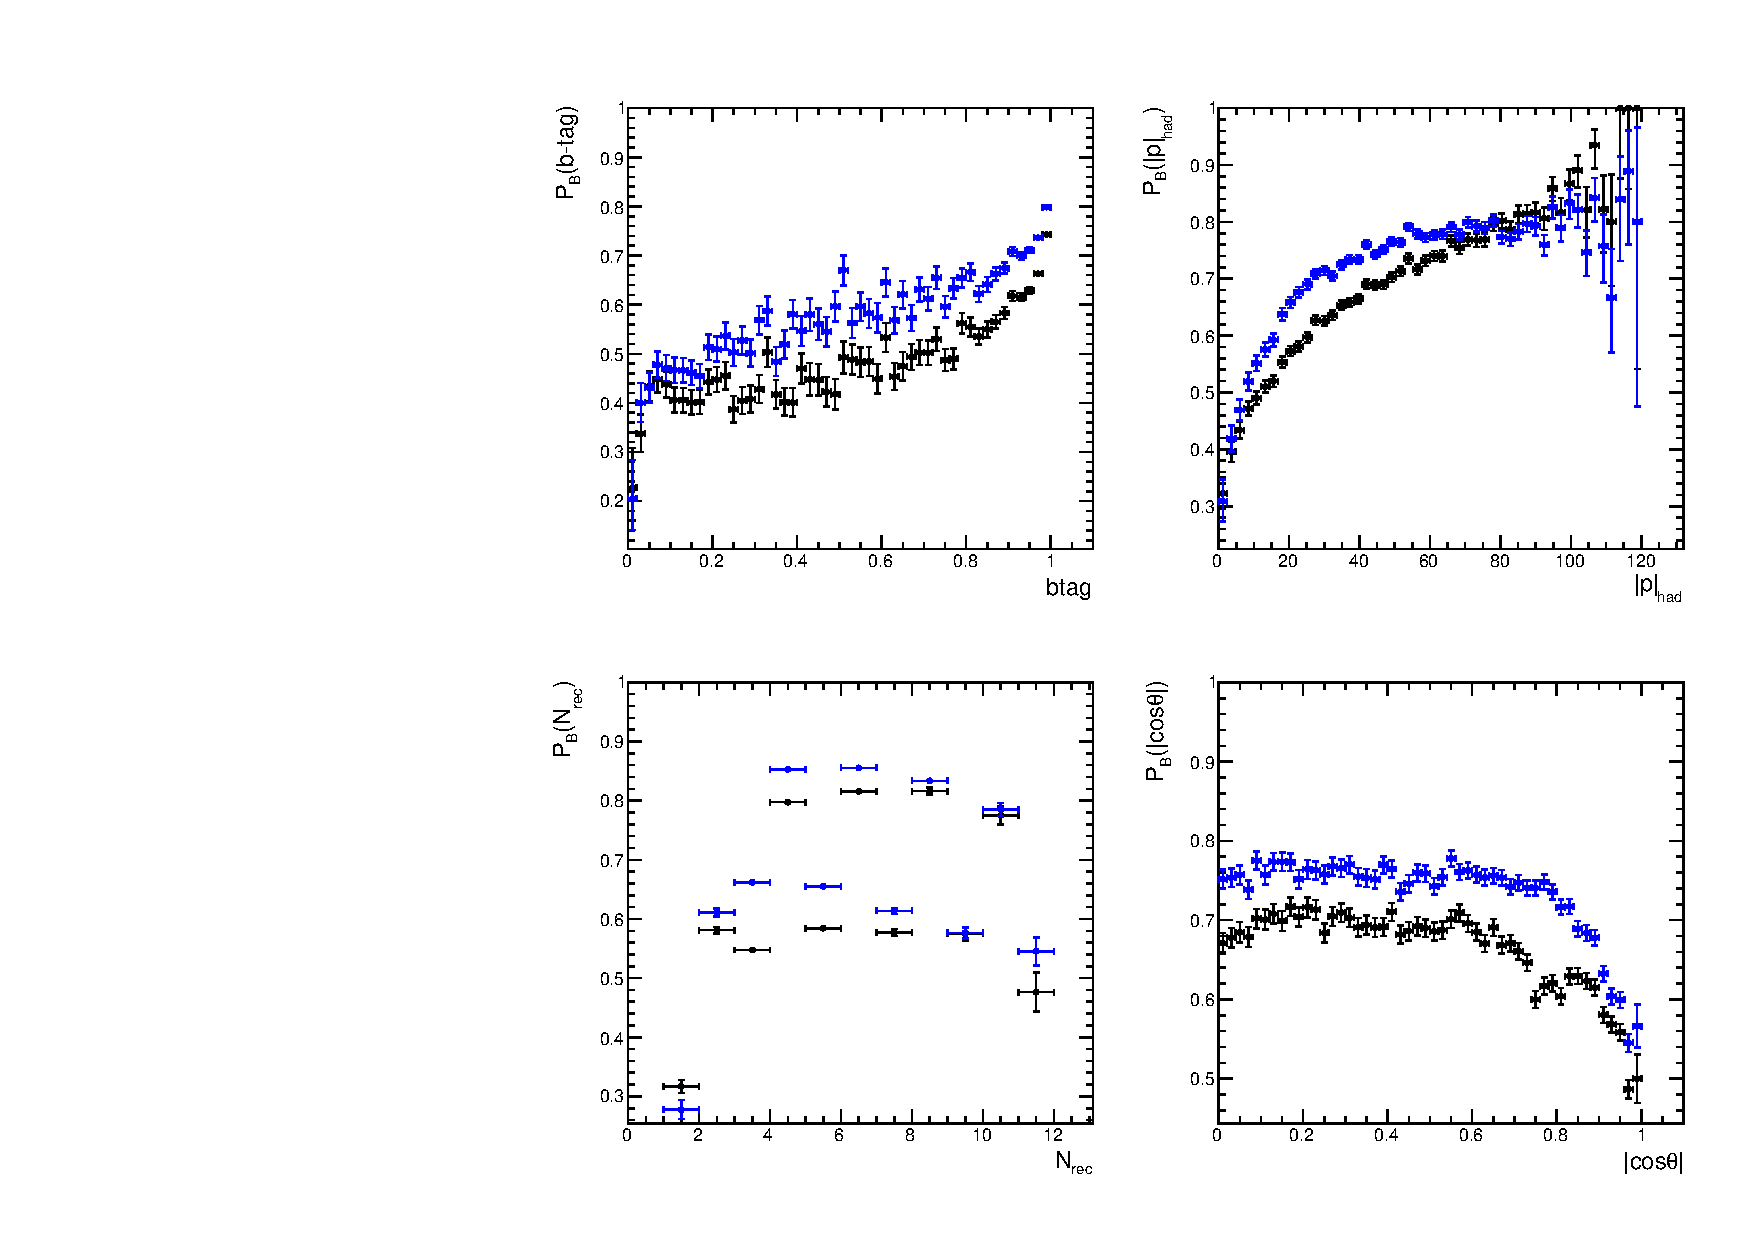
\includegraphics[width=0.95\textwidth]{ILD/plots/recovery-purity-comparison.pdf}
		\caption{\sl Comparaison de la pureté en fonction de b-tag, l'impulsion du hadron de $b$ reconstruit, $N_ {rec}$ et l'angle polaire $|\cos\theta|$ avant et après l'algorithme de récupération de vertex. 
		}
		\label{fig:RecoveryPurityComparison_3F}
	}
\end{figure}

\begin{figure}
	{\centering
		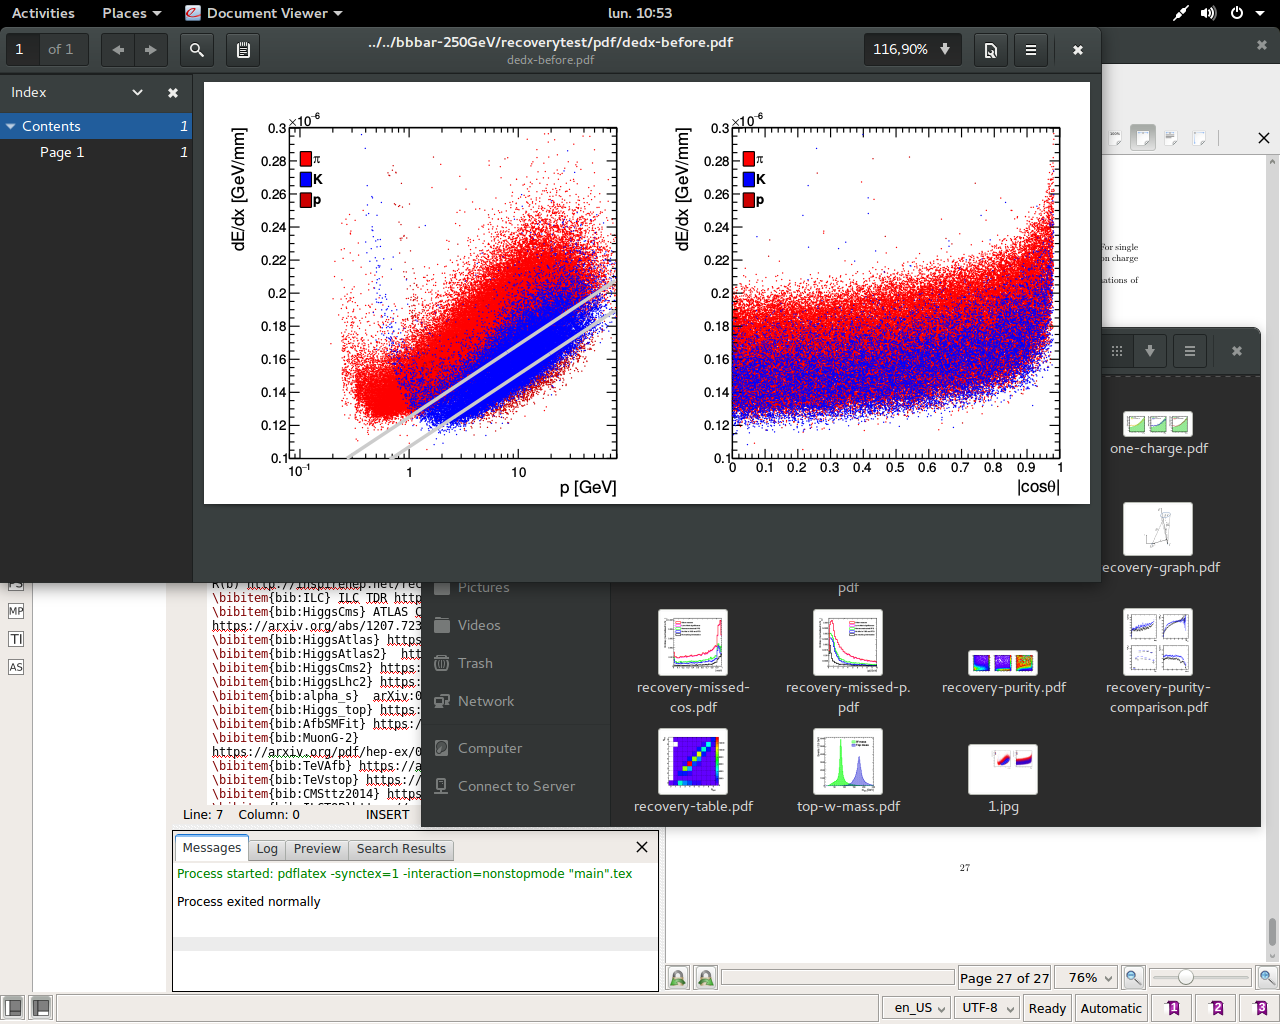
\includegraphics[clip, trim=8cm 18.5cm 7cm 4cm,width=0.95\textwidth]{ILD/plots/dedx-before.png}
		\caption{\sl Le dépôt d'énergie par longueur de trace $dE/dx$ en fonction de l'impulsion des particules, l'angle polaire des particules $|\cos\theta|$ pour pions, kaons et protons. Deux lignes grises séparent la région avec une concentration maximale de kaons.
		}
		\label{fig:dEdxBefore_3F}
	}
\end{figure}

\begin{figure}
	{\centering
		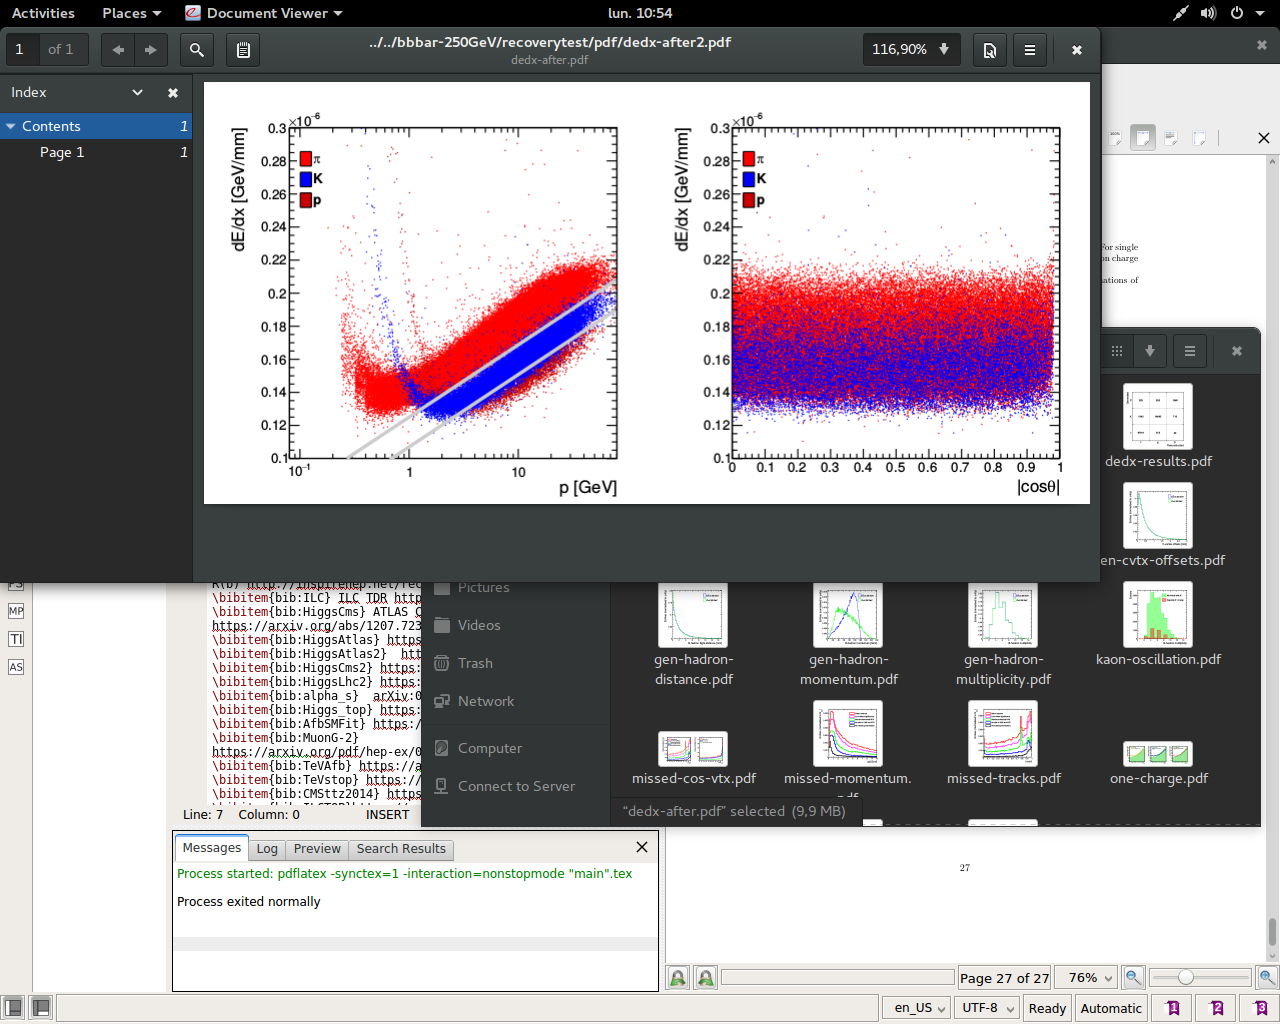
\includegraphics[clip, trim=8cm 18.5cm 7cm 4cm, width=0.95\textwidth]{ILD/plots/dedx-after.png}
		\caption{\sl Le dépôt d'énergie par longueur de trace $dE/dx$ en fonction de l'impulsion des particules, l'angle polaire des particules $|\cos\theta|$ pour pions, kaons et protons. apr\'es l'application de la correction angulaire.  Deux lignes grises séparent la région avec une concentration maximale de kaons.
		}
		\label{fig:dEdxAfter_3F}
	}
\end{figure}


%-----------------------------------------------------------------------------
%-----------------------------------------------------------------------------
%-----------------------------------------------------------------------------
\newpage
\subsection*{Reconstruction de l'angle polaire du quark top et bottom}
L’\'etude du quark top suppose une \'energie dans le centre de masse de $\sqrt{s} = 500$\,GeV et une luminosit\'e int\'egr\'ee de $500$\ifb. L'analyse precendant a \'et\'e fait  en utilisant de methode de la charge de $W^\pm$ lepton~\cite{bib:ILCTOP}.
Dans un premier temps, les nouvelles méthodes ont été appliquées dans le canal semi-leptonique du  quark top pour améliorer l'efficasit\'e de reconstruction de la charge du quark top.
Le resultat après l'application de toutes les combinaisons de paires possibles de la charge de sommet, de la charge de kaon et de la charge de $W^\pm$ lepton à la reconstruction de l'angle polaire supérieur illustrée dans la Fig.~\ref {fig:TopAsymmetryChi_3F}.

%<<<<<<< HEAD
Cette méthode permet de reconstituer l'asymétrie aussi bon que $A_ {FB}^{rec} / A^{gen}_{FB} = 94\%$ avec l'efficacité finale de 38,6\%, ce qui améliore le résultat précédent~\cite{bib:ILCTOP} par 25\%.
%=======
%Cette méthode permet de reconstruire l'asymétrie avant-arriere $A_{FB}$ aussi bon que $A_ {FB}^{rec} / A^{gen}_{FB} = 94\%$ avec l'efficacité finale de 38,6\%, ce qui améliore le résultat précédent~\cite {bib:ILCTOP} par 25\%.
%>>>>>>> 8e36eba08c2388bfd3f0081d6e8eb96636cb3e72

La méthode la plus utilisée est la combinaison de la charge de vertex avec la charge $W^\pm$ lepton car le $ W^\pm$ lepton doit être reconstruit dans chaque événement sélectionné.

\begin{figure}
	\centering
	\begin{subfigure}{0.5\textwidth}
		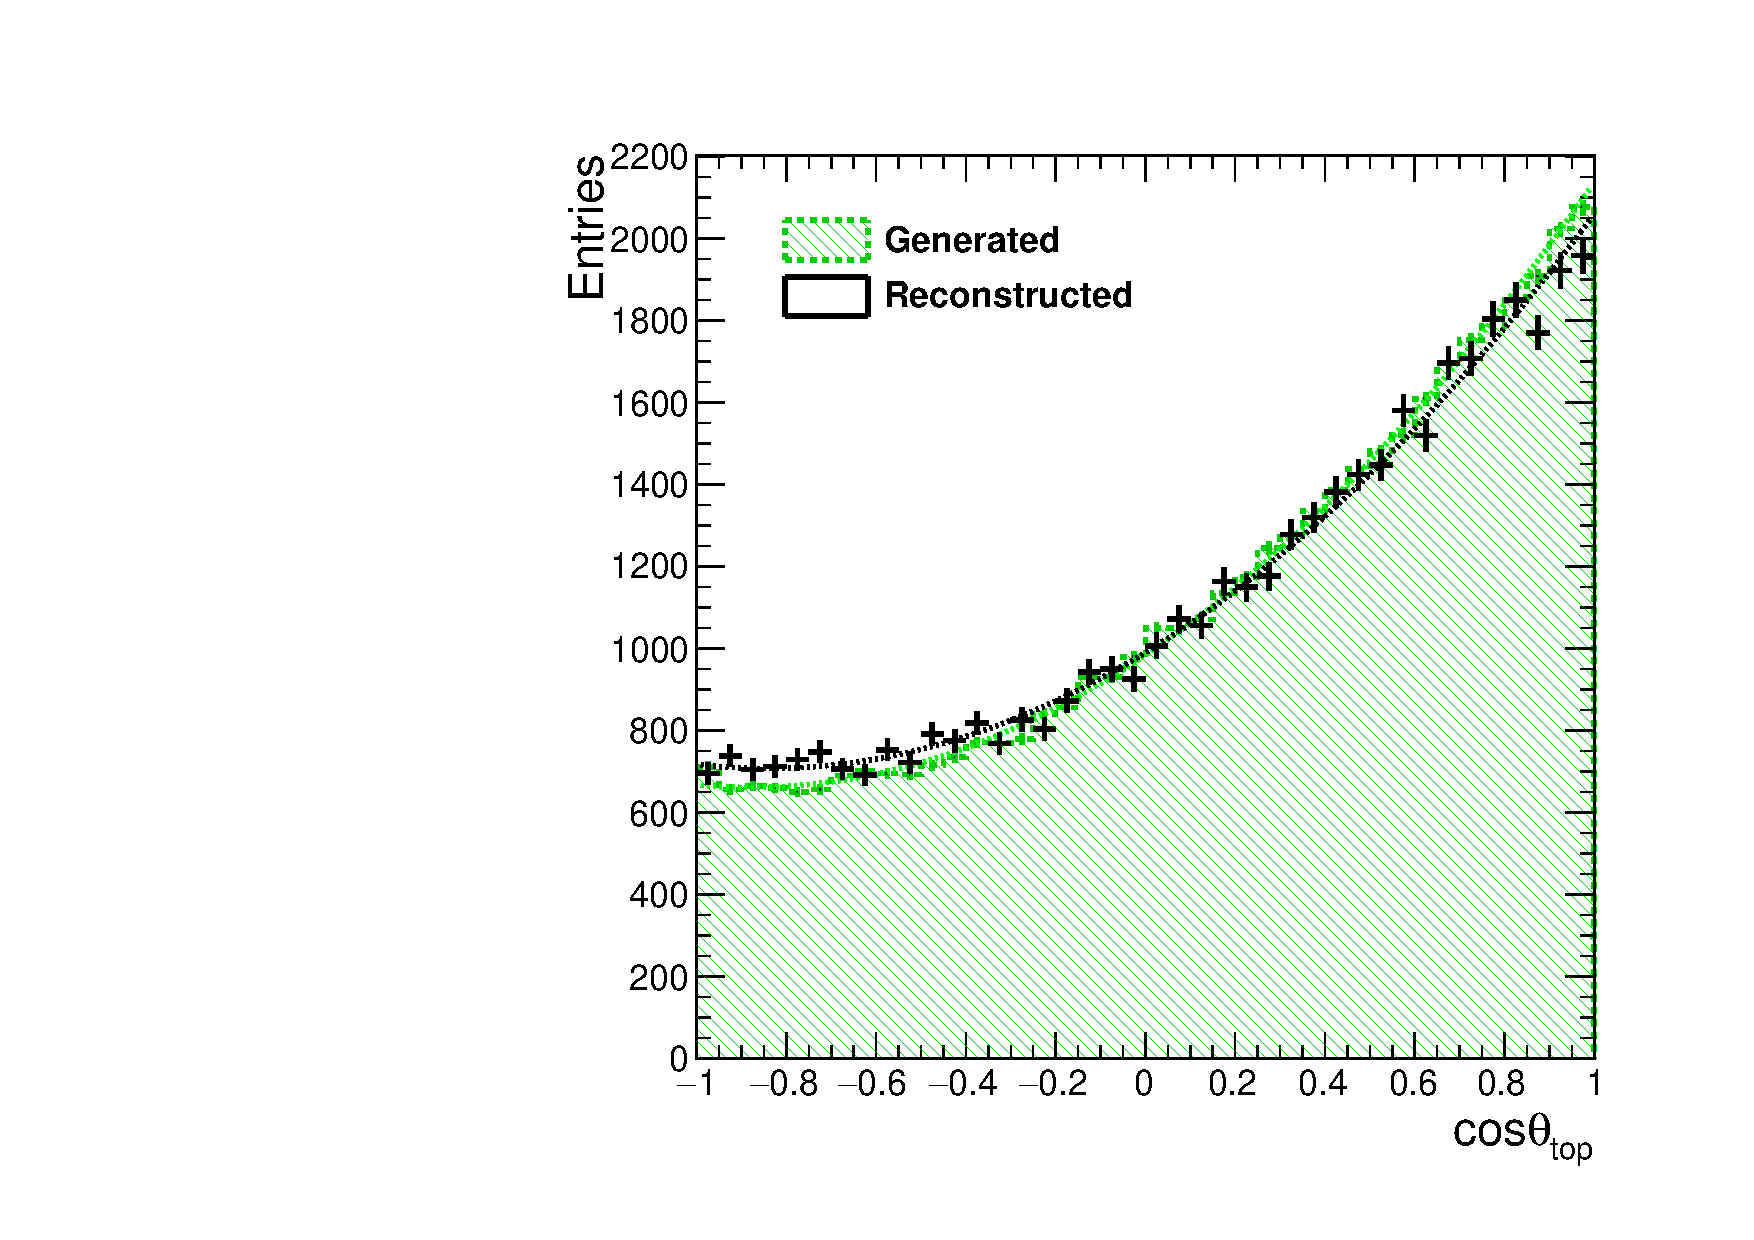
\includegraphics[width=0.95\textwidth]{ILD/plots/top-asymmetry-lepton.pdf}
		\caption{\label{fig:TopAsymmetryChi_a_3F} }
	\end{subfigure}% 
	\begin{subfigure}{0.5\textwidth}
		\centering
		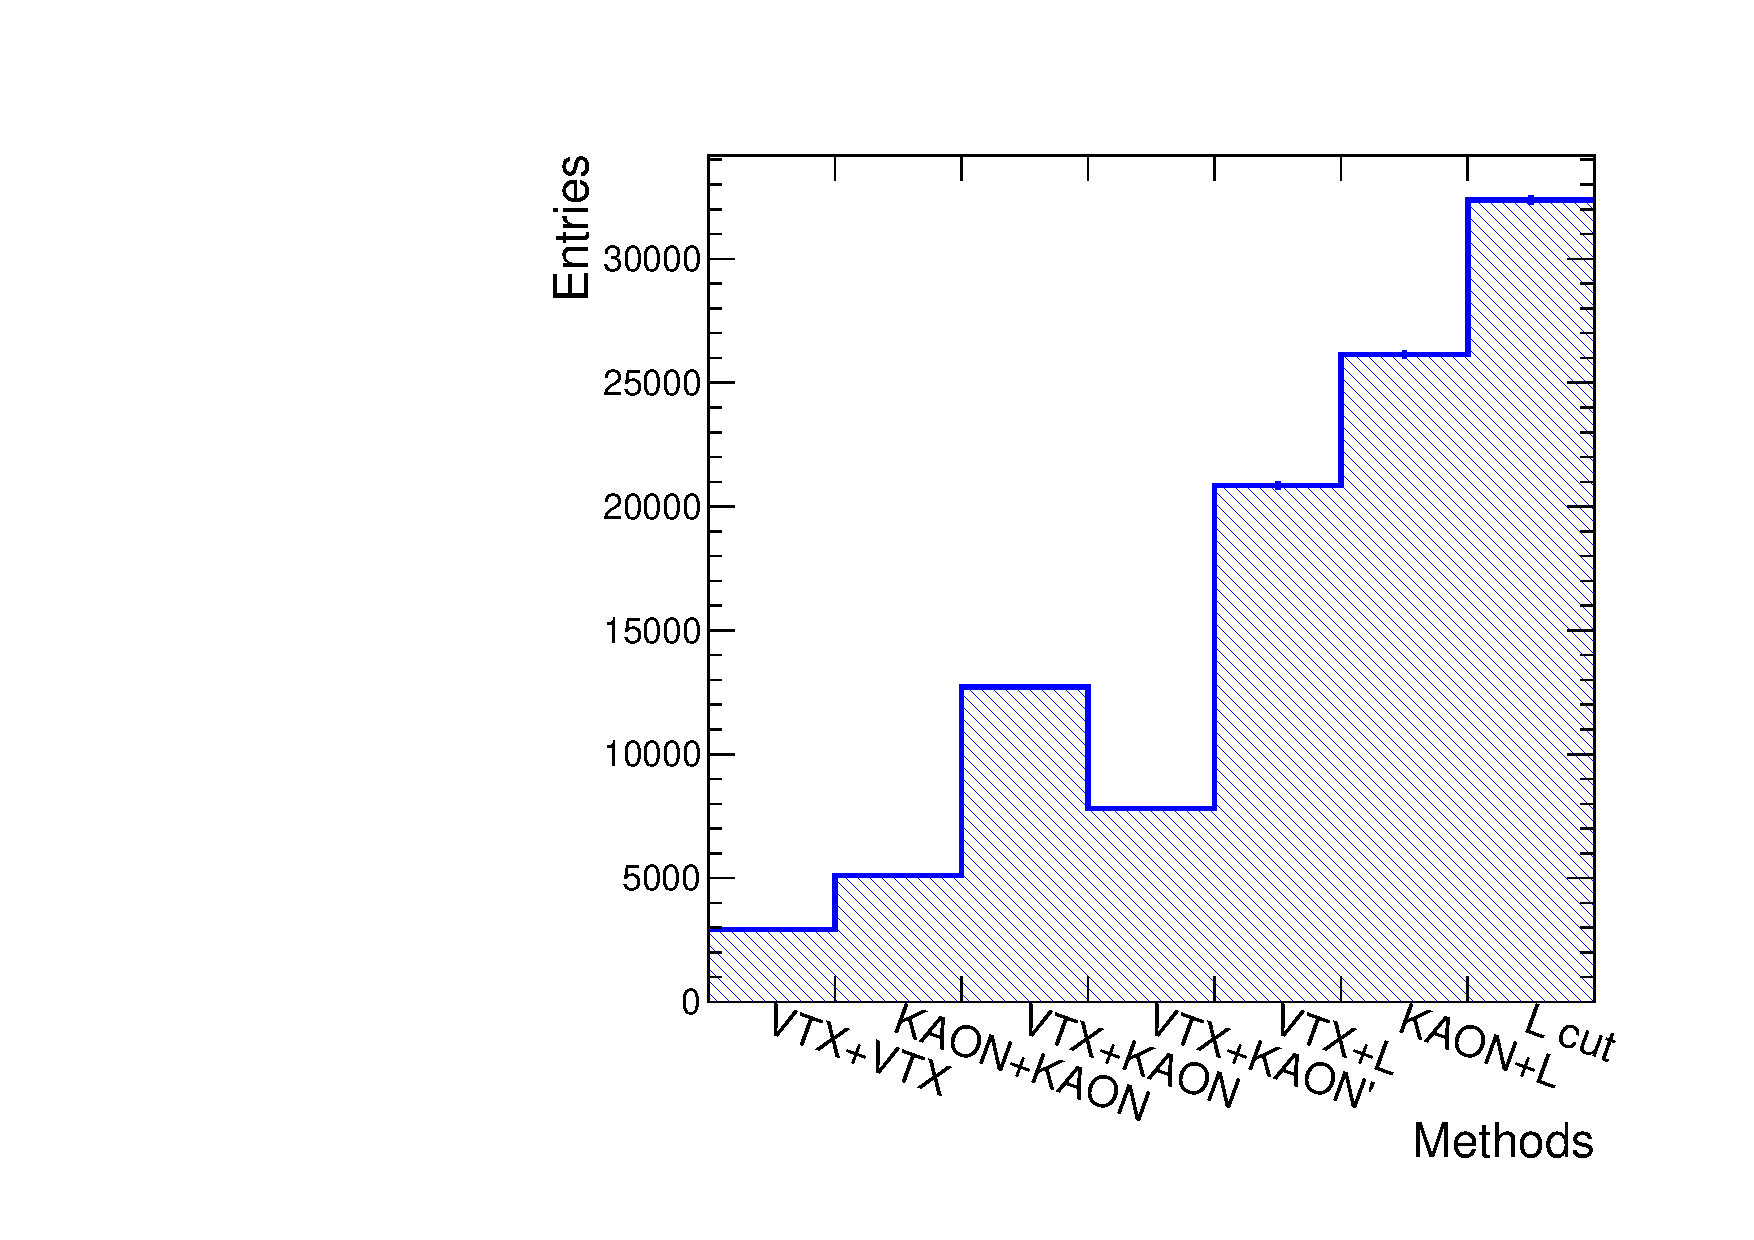
\includegraphics[width=0.95\textwidth]{ILD/plots/top-methods-lepton.pdf}
		\caption{\label{fig:TopAsymmetryChi_b_3F} }
	\end{subfigure}
	\caption{\sl Répartition de l'angle polaire générée par rapport à l'angle polaire reconstruit (a) du quark top en utilisant toutes les combinaisons possibles de signature de charge, tracée en (b).}
	\label{fig:TopAsymmetryChi_3F}
\end{figure}

%-----------------------------------------------------------------------------
%-----------------------------------------------------------------------------
%-----------------------------------------------------------------------------
En suit, on peux appliquer les nouvelles methodes pour reconstruction des couplages \'electrofaibles de la quark $b$. 
Les spectres de l'angle polaire reconstruits du quark $b$ à $\sqrt{s} = 250$\,GeV utilisant une combinaison de signatures des charges des kaons et du vertex sont affich\`ees dans la Fig. ~\ref{fig:BAsymmetryFinal_3F}. La luminosité intégrée $\mathcal{L}_I=250$\,fb$^{-1}$ est supposée pour chaque polarisation du faisceau.

%\subsection*{Reconstruction de l'angle polaire du quark bottom et top}

\begin{figure}
	\centering
	\begin{subfigure}{0.5\textwidth}
		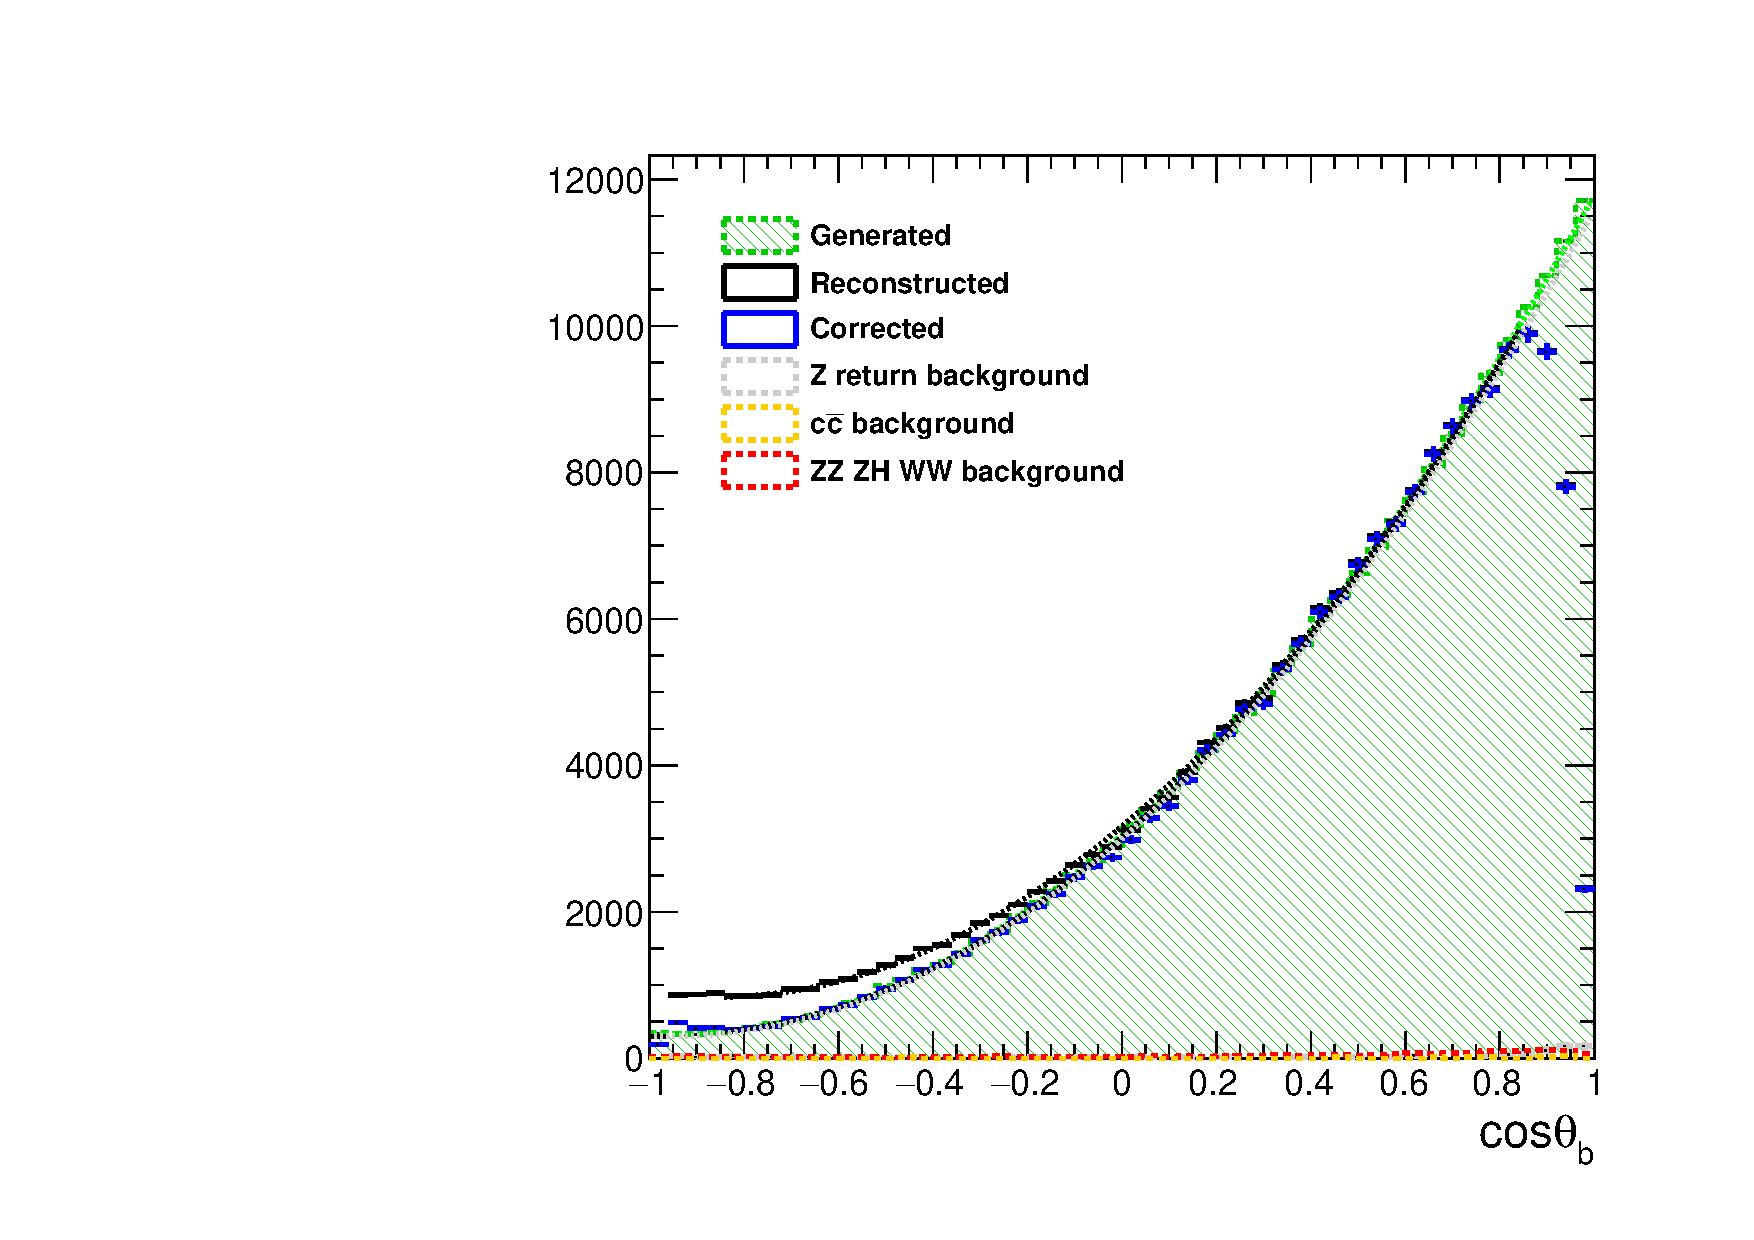
\includegraphics[width=0.95\textwidth]{ILD/plots/basymmetry-final-left.pdf}
		\llap{\shortstack{%
				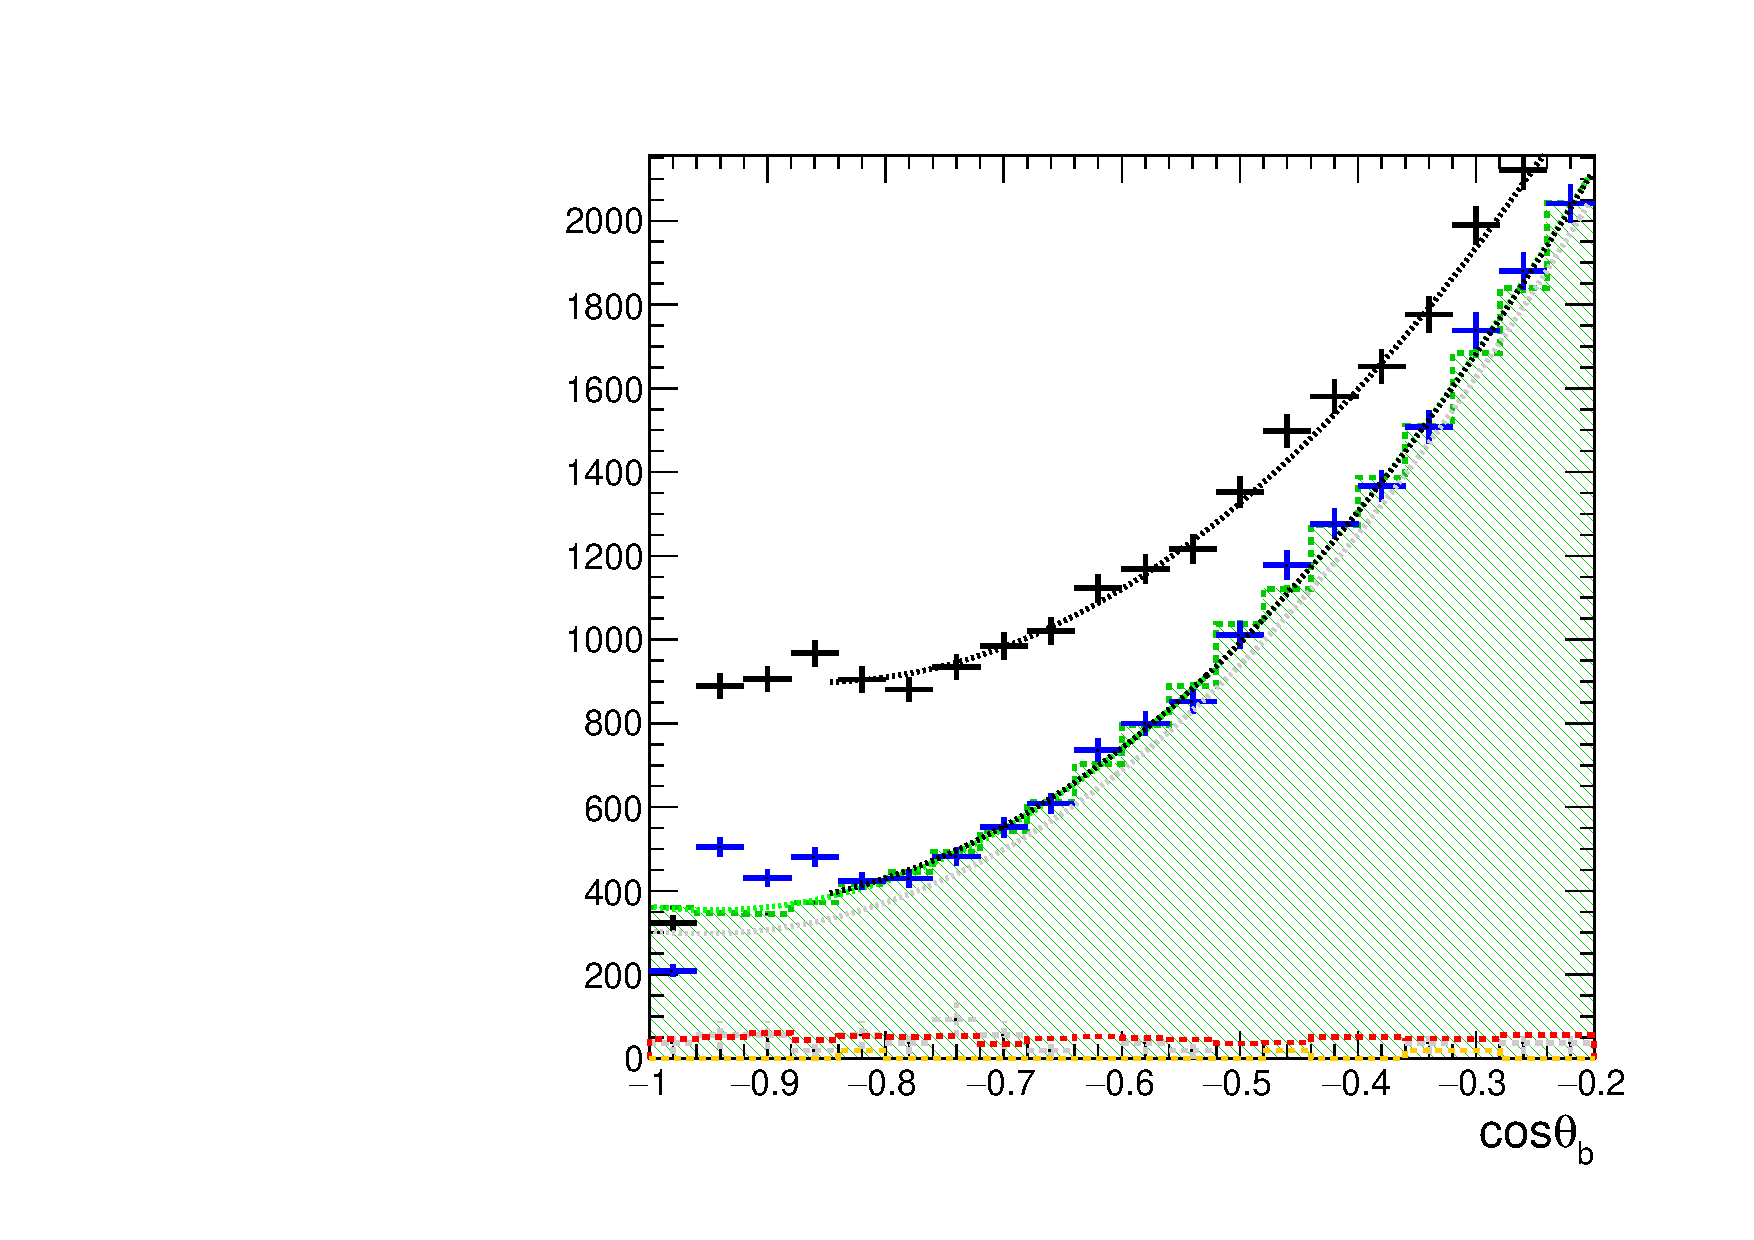
\includegraphics[clip, trim=0cm 0cm 1.8cm 1.7cm, scale=.14]{ILD/plots/zoom-final.pdf}\\
				\rule{0ex}{0.38in}%
			}
			\rule{1.8in}{0ex}}
		\caption{\label{fig:BAsymmetryFinal_a_3F} }
	\end{subfigure}% 
	\begin{subfigure}{0.5\textwidth}
		\centering
		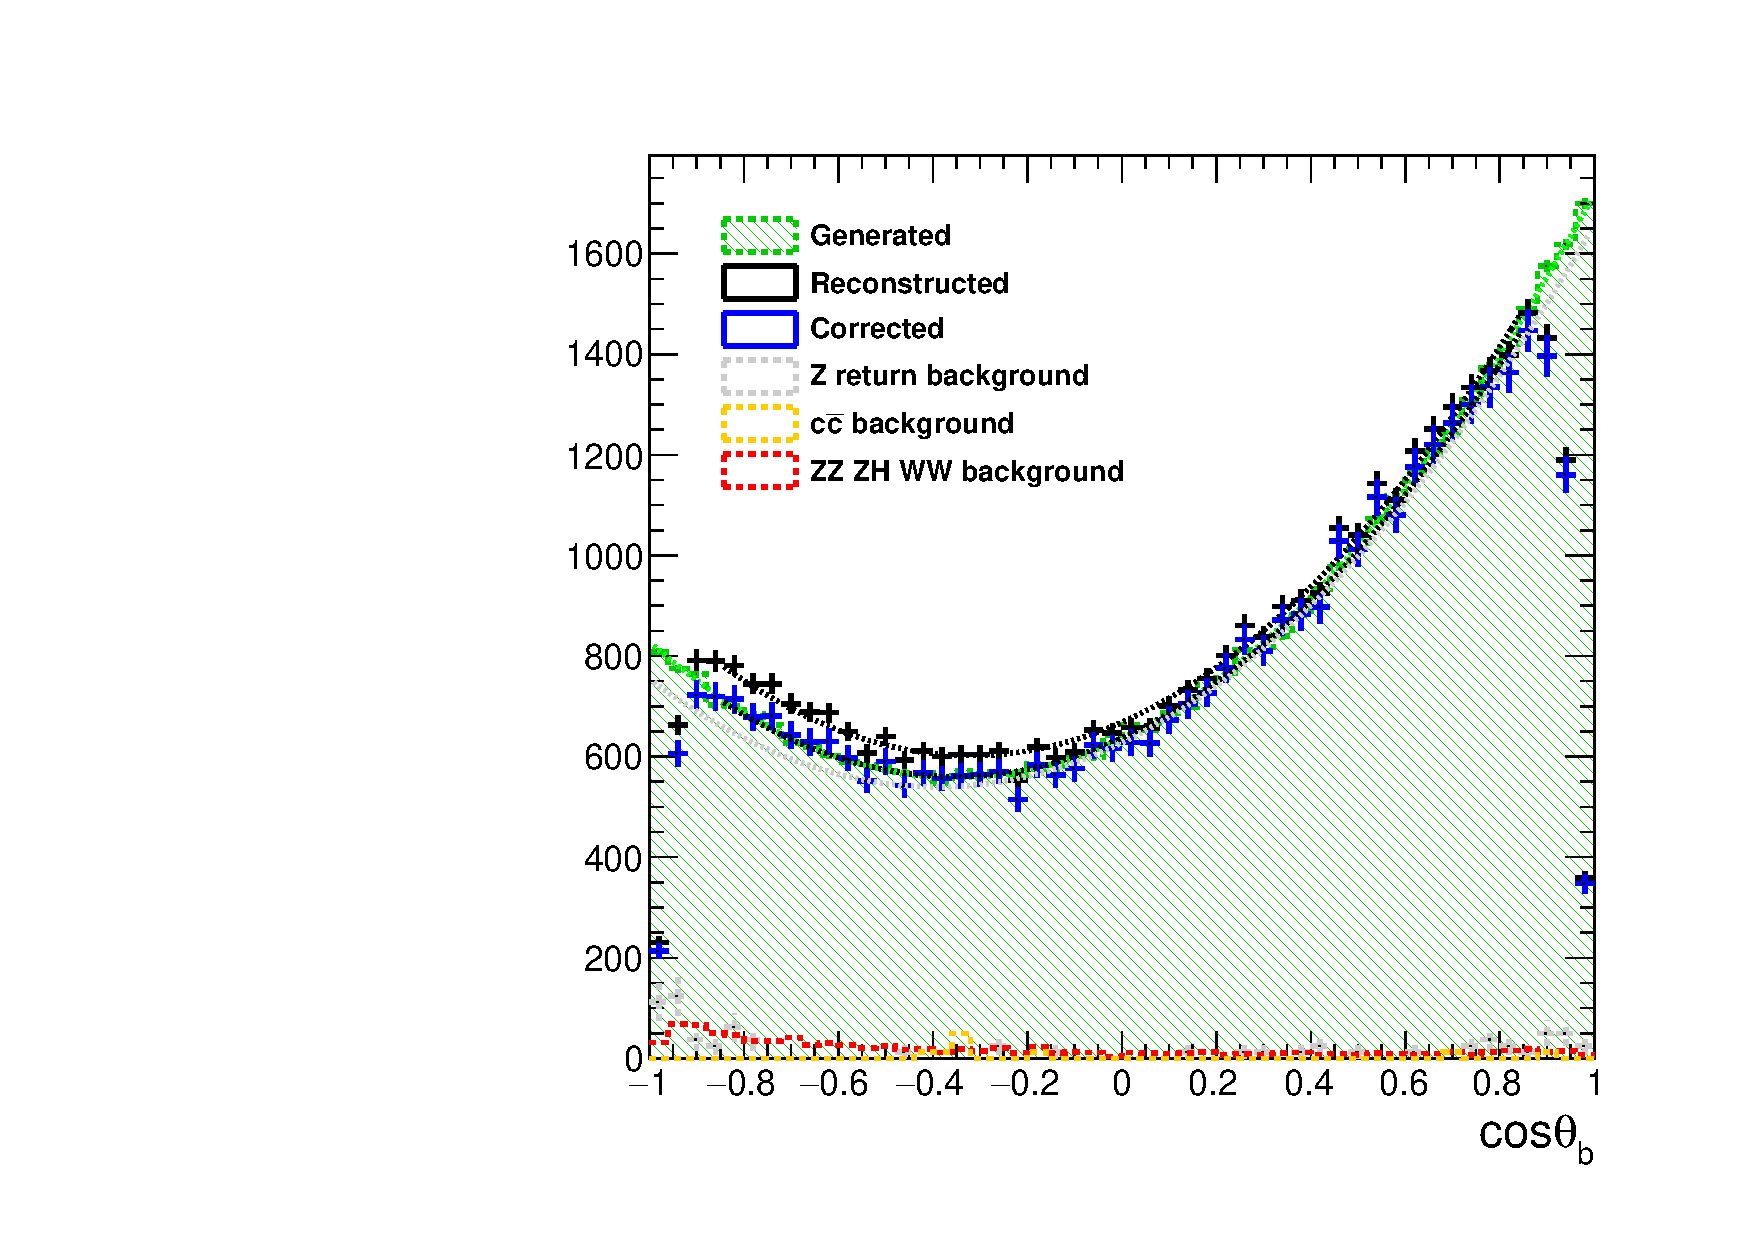
\includegraphics[width=0.95\textwidth]{ILD/plots/basymmetry-final-right.pdf}
		\caption{\label{fig:BAsymmetryFinal_b_3F} }
	\end{subfigure}
	\caption{\sl Distributions de l'angle polaire des quarks b générée comparées aux distrbutions de l'angle polaire des quarks b reconstruites pour la configuration $P_{e}-=-1, P_{e^+}=+1$ (a) et $P_{e}-=+1, P_{e^+}=-1$(b) les processus de fond sont superposés.}
	\label{fig:BAsymmetryFinal_3F}
\end{figure}

Le spectre final est obtenu par une correction supplémentaire qui se sert des mesures contradictoires des charges sans faisant appel à l'information du générateur.  % En utilisant les puretés mesurées, le spectre reconstruit est corrigé à l'aide d'une procédure basée sur les données.
Les distributions corrigées sont ajustées par $S(1+\cos^2\theta) + A\cos\theta$ inspiré par Eq.~\ref{formula:DiffSigma_3F}. Les parametres $S$ et $A$ sont donc liés au constants de couplage. 
%La précision extraite sur les paramètres $S$ et $A$ est extrapolée à la polarisation réaliste $\pm 0.8, \mp 0.3$ et à le répartition de la luminosité du programme de physique de l'ILC.
Comme on peut le voir à partir dans la Fig.~\ref{fig:BAsymmetryFinal_3F}, la contribution des processus de fond, comme cf. celle de la production d'un pair de bosons est faible.


Les précisions relatives sur les couplages $Z^0 b\bar{b}$, $g_L^Z$ et $g_R^Z$, pour les mesures LEP~I et pour les performances ILC attendues sont affichées dans la Fig.~\ref{fig:LEPILCResult_3F}.
La précision de l'ILC sur la couplage $g_R^Z$ est suffisante pour confirmer ou rejeter complètement l'influence de la nouvelle physique sur les couplages électrofaibles du quark $b$.

\begin{figure}
	\centering
	\begin{subfigure}{0.5\textwidth}
		\includegraphics[width=0.99\textwidth]{ILD/plots/lep-result-zoom.pdf}
		\caption{\label{fig:LEPILCResult_a_3F} }
	\end{subfigure}% 
	\begin{subfigure}{0.5\textwidth}
		\centering
		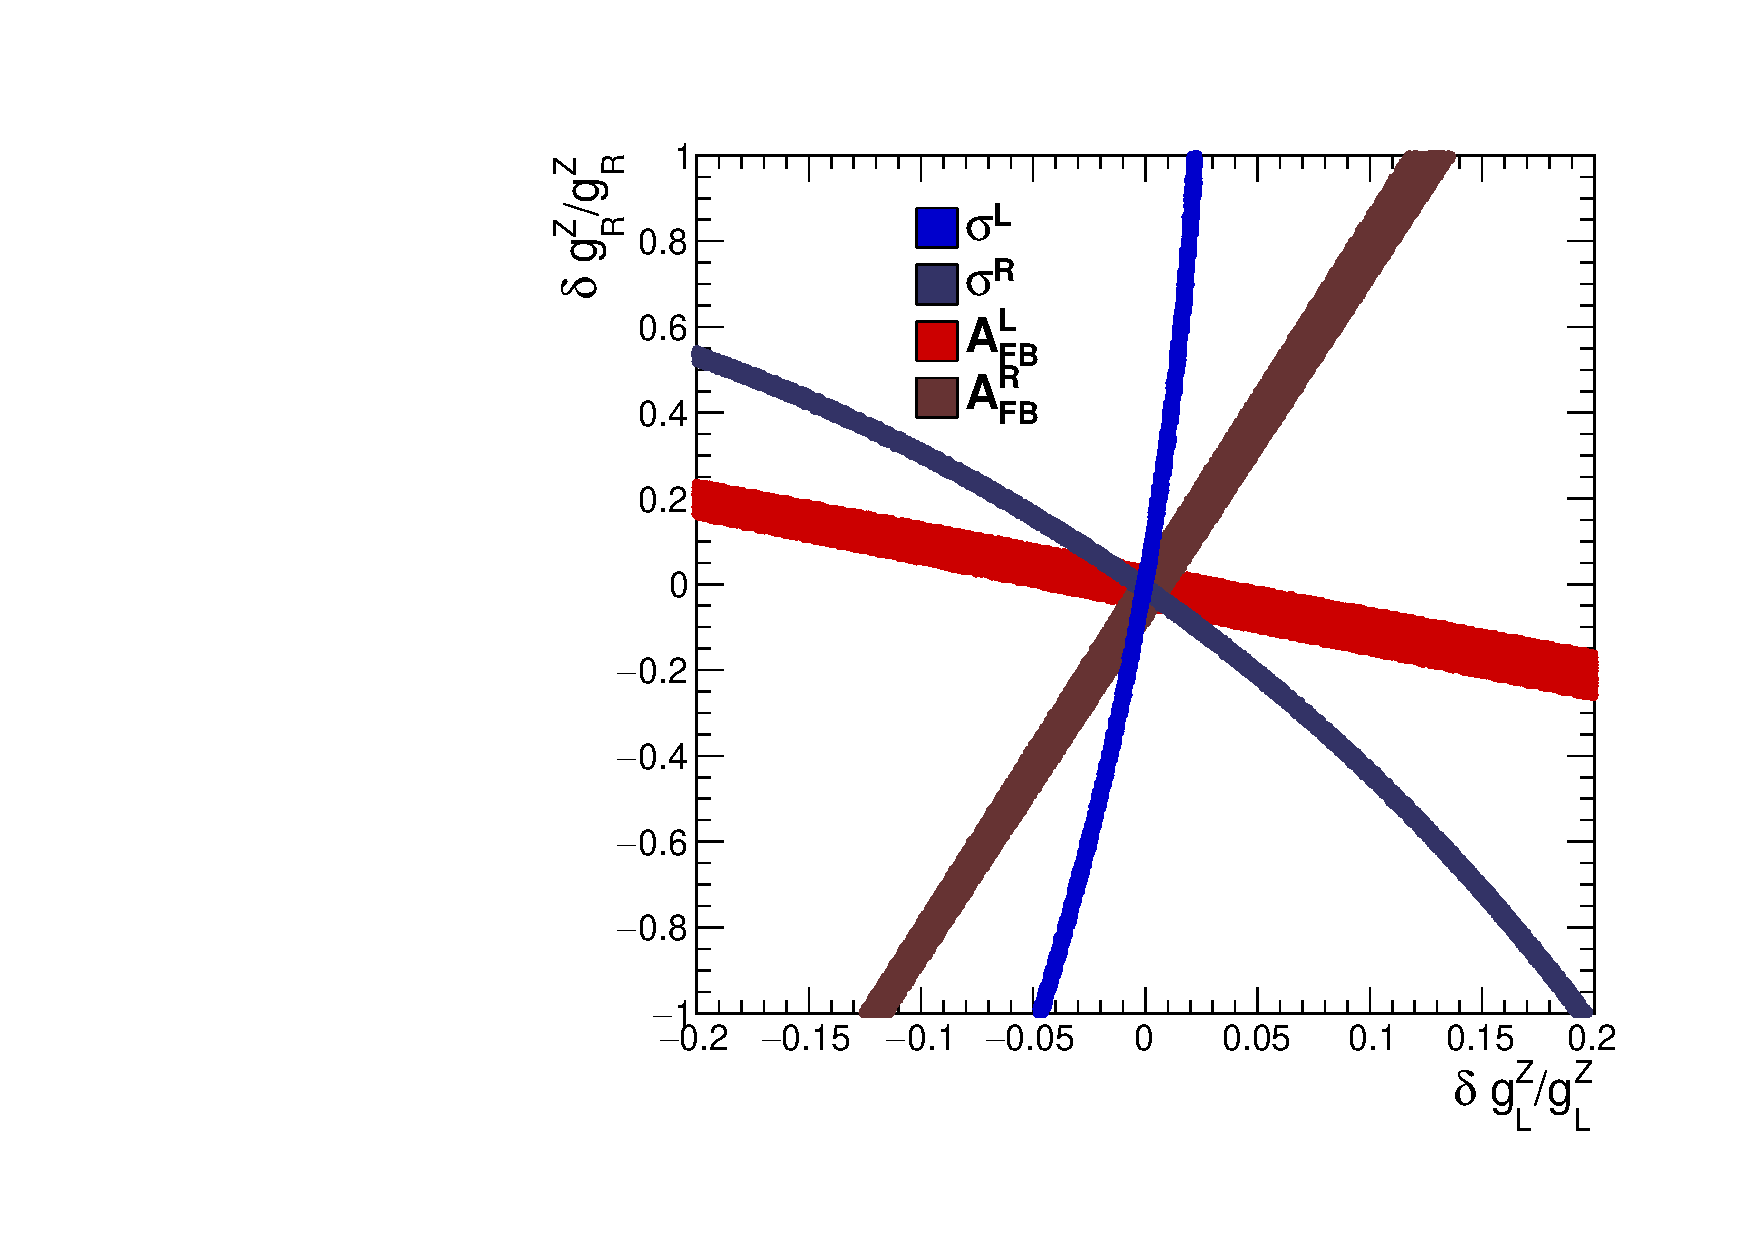
\includegraphics[width=0.99\textwidth]{ILD/plots/ilc-result.pdf}
		\caption{\label{fig:LEPILCResult_b_3F} }
	\end{subfigure}
	\caption{\sl Les régions de $\pm 1\,\sigma$ sur les couplages $Z^0b\bar{b}$ définies par l'asymétrie avant-arrière et les mesures des sections efficaces totales au LEP (a) et à l'ILC via l'ajustement de la section transversale différentielle (b). Les lignes directrices détaillées montrent la valeur \sm. Quant à l'ILC les bandes d'erreurs se chevauchent aux valeurs des couplages attendues par le Modèle standard.  }
	\label{fig:LEPILCResult_3F}
\end{figure}

\subsection*{Conclusions}

Cette thèse présente de nouvelles méthodes et études développées pour l'analyse de données qui seront enregistrées avec les detecteurs au sein de l'ILC. 
D'une cote ces détecteurs sont conçus pour l'application d'algorithmes de flux de particules, qui améliorent la reconstruction des etats finaux des collisions $e^+e^-$ en utilisant les informations des calorimètres hautement granulaires.
A l'autre coté ces detecteurs sont egalement conçus pour une mesure superbe des vertex secondaires.

Le prototype du calorim\`etre \'electromagn\'etique hautement granulaire a été construit et testé par la collaboration CALICE.
Au cours de cette thèse, un algorithme de reconstruction des traces a été développé permettant d'étudier pour la première fois des traces secondaires issues des interactions hadroniques dans le prototype SiW-ECAL.
%La simulation de SiW-ECAL a été comparée aux données en utilisant les nouvelles observables de l'algorithme de recherche de traces.
Les données enregistrées avec ce prototype lors des campagnes de test en faisceau sont comparées avec des predictions des modèles des gerbes hadroniques proposés par le logiciel GEANT4. L'algorithme donne accès aux nouvelles observables répresentées par le nombre de traces dans ce resumé. 


Tous les modèles de simulation testés montrent une bonne performance en termes de nouvelles observables.

Dans cette thèse, les spectres de l'angle polaire des quarks top et bottom sont obtenus à l'aide de la charge du quark b.  
Les méthodes développées sont appliquées aux deux canaux $e^+ e^- \to t\bar{t}$ et $e^+ e^- \to b\bar{b}$ processes à $\sqrt {s} = 500$\,GeV et 250\,GeV, respectivement.

La thèse propose des méthodes pour la determination de la charge du quark $b$ avec une haute pureté. Cela permet de reconstruire précisement l'angle polaire du quark $b$ et d'en extraire les couplages électrofaibles du quark $b$ au boson de $Z^0$.% permet de corriger la distribution  de l'angle polaire pour la contamination résiduelle.
En conséquence, l'angle polaire du quark bottom reconstruit est utilisable pour l'extraction des couplages  et des facteurs de forme électrofaibles du quark bottom.
La précision previsible pour l'ILC sur le couplage $g_R$ est 5 fois meilleure que c'\'etait le cas pour LEP. L'anomalie LEP sera soit donc confirmée, soit définitivement écartée.


